%% bare_conf.tex
%% V1.4
%% 2012/12/27
%% by Michael Shell
%% See:
%% http://www.michaelshell.org/
%% for current contact information.
%%
%% This is a skeleton file demonstrating the use of IEEEtran.cls
%% (requires IEEEtran.cls version 1.8 or later) with an IEEE conference paper.
%%
%% Support sites:
%% http://www.michaelshell.org/tex/ieeetran/
%% http://www.ctan.org/tex-archive/macros/latex/contrib/IEEEtran/
%% and
%% http://www.ieee.org/

%%*************************************************************************
%% Legal Notice:
%% This code is offered as-is without any warranty either expressed or
%% implied; without even the implied warranty of MERCHANTABILITY or
%% FITNESS FOR A PARTICULAR PURPOSE! 
%% User assumes all risk.
%% In no event shall IEEE or any contributor to this code be liable for
%% any damages or losses, including, but not limited to, incidental,
%% consequential, or any other damages, resulting from the use or misuse
%% of any information contained here.
%%
%% All comments are the opinions of their respective authors and are not
%% necessarily endorsed by the IEEE.
%%
%% This work is distributed under the LaTeX Project Public License (LPPL)
%% ( http://www.latex-project.org/ ) version 1.3, and may be freely used,
%% distributed and modified. A copy of the LPPL, version 1.3, is included
%% in the base LaTeX documentation of all distributions of LaTeX released
%% 2003/12/01 or later.
%% Retain all contribution notices and credits.
%% ** Modified files should be clearly indicated as such, including  **
%% ** renaming them and changing author support contact information. **
%%
%% File list of work: IEEEtran.cls, IEEEtran_HOWTO.pdf, bare_adv.tex,
%%                    bare_conf.tex, bare_jrnl.tex, bare_jrnl_compsoc.tex,
%%                    bare_jrnl_transmag.tex
%%*************************************************************************

% *** Authors should verify (and, if needed, correct) their LaTeX system  ***
% *** with the testflow diagnostic prior to trusting their LaTeX platform ***
% *** with production work. IEEE's font choices can trigger bugs that do  ***
% *** not appear when using other class files.                            ***
% The testflow support page is at:
% http://www.michaelshell.org/tex/testflow/



% Note that the a4paper option is mainly intended so that authors in
% countries using A4 can easily print to A4 and see how their papers will
% look in print - the typesetting of the document will not typically be
% affected with changes in paper size (but the bottom and side margins will).
% Use the testflow package mentioned above to verify correct handling of
% both paper sizes by the user's LaTeX system.
%
% Also note that the "draftcls" or "draftclsnofoot", not "draft", option
% should be used if it is desired that the figures are to be displayed in
% draft mode.
%
\documentclass[conference]{IEEEtran}
% Add the compsoc option for Computer Society conferences.
%
% If IEEEtran.cls has not been installed into the LaTeX system files,
% manually specify the path to it like:
% \documentclass[conference]{../sty/IEEEtran}



% Some very useful LaTeX packages include:
% (uncomment the ones you want to load)


% For directly writing german umlauts uncomment the appropriate line for
% your operating system:
% Windows:
% \usepackage[ansinew]{inputenc}
% Linux:
\usepackage[latin1]{inputenc}
% Mac
% \usepackage[applemac]{inputenc}
% If none of the above lines work you can also try the following:
% \usepackage[utf8]{inputenc}



% *** MISC UTILITY PACKAGES ***
%
%\usepackage{ifpdf}
% Heiko Oberdiek's ifpdf.sty is very useful if you need conditional
% compilation based on whether the output is pdf or dvi.
% usage:
% \ifpdf
%   % pdf code
% \else
%   % dvi code
% \fi
% The latest version of ifpdf.sty can be obtained from:
% http://www.ctan.org/tex-archive/macros/latex/contrib/oberdiek/
% Also, note that IEEEtran.cls V1.7 and later provides a builtin
% \ifCLASSINFOpdf conditional that works the same way.
% When switching from latex to pdflatex and vice-versa, the compiler may
% have to be run twice to clear warning/error messages.





% *** CITATION PACKAGES ***
%
%\usepackage{cite}
% cite.sty was written by Donald Arseneau
% V1.6 and later of IEEEtran pre-defines the format of the cite.sty package
% \cite{} output to follow that of IEEE. Loading the cite package will
% result in citation numbers being automatically sorted and properly
% "compressed/ranged". e.g., [1], [9], [2], [7], [5], [6] without using
% cite.sty will become [1], [2], [5]--[7], [9] using cite.sty. cite.sty's
% \cite will automatically add leading space, if needed. Use cite.sty's
% noadjust option (cite.sty V3.8 and later) if you want to turn this off
% such as if a citation ever needs to be enclosed in parenthesis.
% cite.sty is already installed on most LaTeX systems. Be sure and use
% version 4.0 (2003-05-27) and later if using hyperref.sty. cite.sty does
% not currently provide for hyperlinked citations.
% The latest version can be obtained at:
% http://www.ctan.org/tex-archive/macros/latex/contrib/cite/
% The documentation is contained in the cite.sty file itself.





% *** GRAPHICS RELATED PACKAGES ***
%
\ifCLASSINFOpdf
  \usepackage[pdftex]{graphicx}
  % declare the path(s) where your graphic files are
  \graphicspath{{figures/}}
  % and their extensions so you won't have to specify these with
  % every instance of \includegraphics
  % \DeclareGraphicsExtensions{.pdf,.jpeg,.png}
\else
  % or other class option (dvipsone, dvipdf, if not using dvips). graphicx
  % will default to the driver specified in the system graphics.cfg if no
  % driver is specified.
  \usepackage[dvips]{graphicx}
  % declare the path(s) where your graphic files are
  \graphicspath{{figures/}}
  % and their extensions so you won't have to specify these with
  % every instance of \includegraphics
  % \DeclareGraphicsExtensions{.eps}
\fi
% graphicx was written by David Carlisle and Sebastian Rahtz. It is
% required if you want graphics, photos, etc. graphicx.sty is already
% installed on most LaTeX systems. The latest version and documentation
% can be obtained at: 
% http://www.ctan.org/tex-archive/macros/latex/required/graphics/
% Another good source of documentation is "Using Imported Graphics in
% LaTeX2e" by Keith Reckdahl which can be found at:
% http://www.ctan.org/tex-archive/info/epslatex/
%
% latex, and pdflatex in dvi mode, support graphics in encapsulated
% postscript (.eps) format. pdflatex in pdf mode supports graphics
% in .pdf, .jpeg, .png and .mps (metapost) formats. Users should ensure
% that all non-photo figures use a vector format (.eps, .pdf, .mps) and
% not a bitmapped formats (.jpeg, .png). IEEE frowns on bitmapped formats
% which can result in "jaggedy"/blurry rendering of lines and letters as
% well as large increases in file sizes.
%
% You can find documentation about the pdfTeX application at:
% http://www.tug.org/applications/pdftex





% *** MATH PACKAGES ***
%
%\usepackage[cmex10]{amsmath}
% A popular package from the American Mathematical Society that provides
% many useful and powerful commands for dealing with mathematics. If using
% it, be sure to load this package with the cmex10 option to ensure that
% only type 1 fonts will utilized at all point sizes. Without this option,
% it is possible that some math symbols, particularly those within
% footnotes, will be rendered in bitmap form which will result in a
% document that can not be IEEE Xplore compliant!
%
% Also, note that the amsmath package sets \interdisplaylinepenalty to 10000
% thus preventing page breaks from occurring within multiline equations. Use:
%\interdisplaylinepenalty=2500
% after loading amsmath to restore such page breaks as IEEEtran.cls normally
% does. amsmath.sty is already installed on most LaTeX systems. The latest
% version and documentation can be obtained at:
% http://www.ctan.org/tex-archive/macros/latex/required/amslatex/math/





% *** SPECIALIZED LIST PACKAGES ***
%
%\usepackage{algorithmic}
% algorithmic.sty was written by Peter Williams and Rogerio Brito.
% This package provides an algorithmic environment fo describing algorithms.
% You can use the algorithmic environment in-text or within a figure
% environment to provide for a floating algorithm. Do NOT use the algorithm
% floating environment provided by algorithm.sty (by the same authors) or
% algorithm2e.sty (by Christophe Fiorio) as IEEE does not use dedicated
% algorithm float types and packages that provide these will not provide
% correct IEEE style captions. The latest version and documentation of
% algorithmic.sty can be obtained at:
% http://www.ctan.org/tex-archive/macros/latex/contrib/algorithms/
% There is also a support site at:
% http://algorithms.berlios.de/index.html
% Also of interest may be the (relatively newer and more customizable)
% algorithmicx.sty package by Szasz Janos:
% http://www.ctan.org/tex-archive/macros/latex/contrib/algorithmicx/




% *** ALIGNMENT PACKAGES ***
%
\usepackage{array}
% Frank Mittelbach's and David Carlisle's array.sty patches and improves
% the standard LaTeX2e array and tabular environments to provide better
% appearance and additional user controls. As the default LaTeX2e table
% generation code is lacking to the point of almost being broken with
% respect to the quality of the end results, all users are strongly
% advised to use an enhanced (at the very least that provided by array.sty)
% set of table tools. array.sty is already installed on most systems. The
% latest version and documentation can be obtained at:
% http://www.ctan.org/tex-archive/macros/latex/required/tools/


% IEEEtran contains the IEEEeqnarray family of commands that can be used to
% generate multiline equations as well as matrices, tables, etc., of high
% quality.




% *** SUBFIGURE PACKAGES ***
%\ifCLASSOPTIONcompsoc
%  \usepackage[caption=false,font=normalsize,labelfont=sf,textfont=sf]{subfig}
%\else
%  \usepackage[caption=false,font=footnotesize]{subfig}
%\fi
% subfig.sty, written by Steven Douglas Cochran, is the modern replacement
% for subfigure.sty, the latter of which is no longer maintained and is
% incompatible with some LaTeX packages including fixltx2e. However,
% subfig.sty requires and automatically loads Axel Sommerfeldt's caption.sty
% which will override IEEEtran.cls' handling of captions and this will result
% in non-IEEE style figure/table captions. To prevent this problem, be sure
% and invoke subfig.sty's "caption=false" package option (available since
% subfig.sty version 1.3, 2005/06/28) as this is will preserve IEEEtran.cls
% handling of captions.
% Note that the Computer Society format requires a larger sans serif font
% than the serif footnote size font used in traditional IEEE formatting
% and thus the need to invoke different subfig.sty package options depending
% on whether compsoc mode has been enabled.
%
% The latest version and documentation of subfig.sty can be obtained at:
% http://www.ctan.org/tex-archive/macros/latex/contrib/subfig/




% *** FLOAT PACKAGES ***
%
%\usepackage{fixltx2e}
% fixltx2e, the successor to the earlier fix2col.sty, was written by
% Frank Mittelbach and David Carlisle. This package corrects a few problems
% in the LaTeX2e kernel, the most notable of which is that in current
% LaTeX2e releases, the ordering of single and double column floats is not
% guaranteed to be preserved. Thus, an unpatched LaTeX2e can allow a
% single column figure to be placed prior to an earlier double column
% figure. The latest version and documentation can be found at:
% http://www.ctan.org/tex-archive/macros/latex/base/


%\usepackage{stfloats}
% stfloats.sty was written by Sigitas Tolusis. This package gives LaTeX2e
% the ability to do double column floats at the bottom of the page as well
% as the top. (e.g., "\begin{figure*}[!b]" is not normally possible in
% LaTeX2e). It also provides a command:
%\fnbelowfloat
% to enable the placement of footnotes below bottom floats (the standard
% LaTeX2e kernel puts them above bottom floats). This is an invasive package
% which rewrites many portions of the LaTeX2e float routines. It may not work
% with other packages that modify the LaTeX2e float routines. The latest
% version and documentation can be obtained at:
% http://www.ctan.org/tex-archive/macros/latex/contrib/sttools/
% Do not use the stfloats baselinefloat ability as IEEE does not allow
% \baselineskip to stretch. Authors submitting work to the IEEE should note
% that IEEE rarely uses double column equations and that authors should try
% to avoid such use. Do not be tempted to use the cuted.sty or midfloat.sty
% packages (also by Sigitas Tolusis) as IEEE does not format its papers in
% such ways.
% Do not attempt to use stfloats with fixltx2e as they are incompatible.
% Instead, use Morten Hogholm'a dblfloatfix which combines the features
% of both fixltx2e and stfloats:
%
% \usepackage{dblfloatfix}
% The latest version can be found at:
% http://www.ctan.org/tex-archive/macros/latex/contrib/dblfloatfix/




% *** PDF, URL AND HYPERLINK PACKAGES ***
%
%\usepackage{url}
% url.sty was written by Donald Arseneau. It provides better support for
% handling and breaking URLs. url.sty is already installed on most LaTeX
% systems. The latest version and documentation can be obtained at:
% http://www.ctan.org/tex-archive/macros/latex/contrib/url/
% Basically, \url{my_url_here}.




% *** Do not adjust lengths that control margins, column widths, etc. ***
% *** Do not use packages that alter fonts (such as pslatex).         ***
% There should be no need to do such things with IEEEtran.cls V1.6 and later.
% (Unless specifically asked to do so by the journal or conference you plan
% to submit to, of course. )


% add custom packages

% lipsum
\usepackage{xcolor}
\usepackage{lipsum}
\setlipsum{%
    par-before = \begingroup\color{lightgray},
    par-after = \endgroup,
    sentence-before = \begingroup\color{lightgray},
    sentence-after = \endgroup
}

\definecolor{tumblue}{rgb}{0, 0.4, 0.74}

\newcommand{\comment}[1]{{\color{tumblue} #1}}



% correct bad hyphenation here
\hyphenation{op-tical net-works semi-conduc-tor}

\usepackage{amsfonts}
\usepackage{amssymb}
\usepackage{amsmath}
\usepackage{amsthm}
\newtheorem{theorem}{Theorem}
\newtheorem{proposition}{Proposition}
\newtheorem{example}{Example}
\newtheorem{definition}{Definition}
\newtheorem{lemma}{Lemma}

\usepackage[colorlinks=true,linkcolor=blue!70!black,
  citecolor=green!50!black,urlcolor=blue!70!black]{hyperref}
\usepackage{cleveref}

\crefname{section}{Sec.}{Sec.}
\crefname{subsection}{Sec.}{Sec.}
\crefname{figure}{Fig.}{Fig.}
\crefname{algorithm}{Alg.}{Alg.}
\crefname{table}{Tab.}{Tab.}
\crefname{example}{Example}{Example}
\crefname{definition}{Def.}{Def.}
\crefname{proposition}{Prop.}{Prop.}
\crefname{theorem}{Thm.}{Thm.}
\crefname{lemma}{Lemma}{Lemmas}

\Crefname{section}{Sec.}{Sec.}
\Crefname{subsection}{Sec.}{Sec.}
\Crefname{figure}{Fig.}{Fig.}
\Crefname{algorithm}{Alg.}{Alg.}
\Crefname{table}{Tab.}{Tab.}
\crefname{example}{Example}{Example}
\Crefname{definition}{Def.}{Def.}
\Crefname{proposition}{Prop.}{Prop.}
\Crefname{theorem}{Thm.}{Thm.}
\Crefname{lemma}{Lemma}{Lemmas}

\usepackage{booktabs} % professional tables
\usepackage{multirow}


% tikz
% you can export matlab figures directly to latex/tikz using the following setup.
% Ask your supervisor for access to our matlab2tikz repository if you want to use it
% Important: You have to add --shell-escape to your latex call for tikz externalization to work properly
\usepackage{tikzscale}
\usepackage{pgfplots}
\usepackage{mathtools}
\pgfplotsset{compat=1.18}
\usepgfplotslibrary{external}
%\tikzexternalize[prefix=./figures/externalize/]
%\newcommand{\includetikz}[1]{%
%    \tikzsetnextfilename{#1}%
%    \input{#1.tikz}%
%}
% explicitly set line width to avoid different widths in different pdf viewers
\tikzset{every picture/.style={line width=0.5pt}}
% groupplots
\usepgfplotslibrary{groupplots}
\usetikzlibrary{pgfplots.groupplots}
\usetikzlibrary{matrix}


% for operators and sets
\newcommand{\operator}[2]{\text{\normalfont\small\texttt{#1}}\left(#2\right)}
\newcommand{\opDiag}[1]{\operator{diag}{#1}}

\usepackage{xifthen}
\newcommand{\negphantom}[1]{\settowidth{\dimen0}{#1}\hspace*{-\dimen0}} % used to position punctuation neatly
\newcommand{\defSet}[3][2]{\left<#3\right>_{#2}\ifthenelse{\isempty{#1}}{}{\negphantom{#2}#1\phantom{\scriptstyle #2}}}
\newcommand{\defSetAligned}[3]{\begin{split}#2 = \left<#3\right>_{#1}\end{split}}

% Additional packages and commands for the BNN report
\usepackage{bm}
\usepackage{float}
\usepackage{enumitem}
\usepackage{listings}
\usepackage{caption}
\usepackage{subcaption}
\usepackage{rotating}
\usepackage[numbers,sort&compress]{natbib}
\usepackage{fancyhdr}
\usepackage{parskip}

\definecolor{codebg}{RGB}{248,248,248}
\lstdefinestyle{pythonstyle}{
  backgroundcolor=\color{codebg},basicstyle=\ttfamily\small,
  keywordstyle=\bfseries,frame=single,breaklines=true,
  language=Python,showstringspaces=false,
  numbers=left,numberstyle=\tiny\color{gray},xleftmargin=2em}
\lstset{style=pythonstyle}

\newcommand{\btheta}{\bm{\theta}}
\newcommand{\cD}{\mathcal{D}}
\newcommand{\cN}{\mathcal{N}}
\newcommand{\KL}{\mathrm{KL}}
\newcommand{\ELBO}{\mathcal{L}_{\text{ELBO}}}
\newcommand{\MAP}{\text{MAP}}
\newcolumntype{C}[1]{>{\centering\arraybackslash}p{#1}}
\newcolumntype{L}[1]{>{\raggedright\arraybackslash}p{#1}}

\raggedbottom

\begin{document}

% Add the seminar's cover page
\begin{figure*}[!h]

  \includegraphics{./figures/IN.pdf} \hfill \includegraphics{./figures/tumlogo.pdf}
 
  \vspace*{1cm}
  {\large \textsf{TUM School of Computation, Information and Technology}}\\
  {\large \textsf{Professorship of Cyber Physical Systems}}\\
   

  \vspace*{5cm}
%
%
% TITEL DER ARBEIT
%
%
  {\color{tumblue} \Huge \bf \textsf{Bayesian Neural Networks:
Implementations using Python Libraries}}\\  % HIER EINSETZEN!

  \vspace*{1cm}
%
%
% NAME DES STUDENTEN (auf Titelblatt)
%
% 
  {\Large \bf \textsf{Gabriel Gerardo Carpio Saez de Nanclares}}\\   % HIER EINSETZEN!
 
  \vspace*{8cm}
  {\Large \textsf{Practical Course: \emph{Formal Methods for AI-Enabled Cyber-Physical Systems} - SS 2026}}\\
 
  \vspace*{1cm} 
  \begin{tabular}{ll}
%
%
% NAME DES BETREUERS
%
%
    {\Large \bf \textsf{Advisor:}} &
    {\Large \textsf{Laura Lützow \& Victor Schulte}}\\                  % HIER EINSETZEN!
    \\

    {\Large \bf \textsf{Supervisor:}} &
    {\Large \textsf{Prof.~Dr.-Ing. Matthias Althoff}}\\
    \\

%
%
% ABGABETERMIN
%
%
    {\Large \bf \textsf{Submission:}} &
    {\Large \textsf{01. January 2025}}

  \end{tabular}
  
\end{figure*}


%
% paper title
% can use linebreaks \\ within to get better formatting as desired
% Do not put math or special symbols in the title.
\title{Bayesian Neural Networks:\\[4pt] Implementations using Python Libraries}


% author names and affiliations
% use a multiple column layout for up to three different
% affiliations
\author{\IEEEauthorblockN{Gabriel Gerardo Carpio Saez de Nanclares}
	\IEEEauthorblockA{Technische Universit\"at M\"unchen\\
		Email: go82duw@mytum.de}}

% conference papers do not typically use \thanks and this command
% is locked out in conference mode. If really needed, such as for
% the acknowledgment of grants, issue a \IEEEoverridecommandlockouts
% after \documentclass

% use for special paper notices
%\IEEEspecialpapernotice{(Invited Paper)}



% make the title area
\maketitle

% As a general rule, do not put math, special symbols or citations
% in the abstract
\begin{abstract}
    A way of addressing uncertainty in Deep Learning is through Bayesian Neural Networks. Two ways
    of implementing them are through Variational Inference and the Laplace Approximation. This report
    compares two PyTorch libraries implementing these paradigms: \texttt{bayesian-torch} and
    \texttt{laplace-torch}. Experiments span classification and regression tasks, where different possible
    configurations are explored. The results show that the Laplace Approximation is a more efficient method,
    as it takes less time to train and at inference as well, while still performing well in the metrics used
    for evaluating the uncertainty against the true accuracy of the models. \texttt{bayesian-torch} still performs
    very well, but the results when analysing Out of Distribution testing show that this approach might be
    ill-suited for such a task. The discussion explores the future work, suggesting that a proper analysis of OOD
    detection is needed to further understand these methods.
\end{abstract}

% no keywords




% For peer review papers, you can put extra information on the cover
% page as needed:
% \ifCLASSOPTIONpeerreview
% \begin{center} \bfseries EDICS Category: 3-BBND \end{center}
% \fi
%
% For peerreview papers, this IEEEtran command inserts a page break and
% creates the second title. It will be ignored for other modes.
\IEEEpeerreviewmaketitle


\section{Introduction}
\label{sec:intro}

Standard Neural Networks are trained on given datasets in a frequentist manner, and their
point-estimate outputs carry no calibrated notion of confidence. This, together with the
fact that the parameters set during training are deterministic, leads to
over-confidence~\citep{goan2020bayesian,murphy2023pml}. Bayesian Deep Learning (BDL)
addresses this by replacing a deterministic
weight estimate with a posterior distribution $p(\btheta \mid \cD)$, propagating weight
uncertainty into calibrated predictive distributions. This report compares two PyTorch
libraries implementing complementary Bayesian Neural Networks (BNNs) paradigms
(repositories in Section~\ref{sec:software}):
\begin{itemize}[leftmargin=*]
	\item \texttt{bayesian-torch}, a
	      Bayesian by design library from Intel Labs implementing mean field
	      Variational Inference via Flipout~\citep{wen2018flipout} and
	      Bayes by Backprop~\citep{blundell2015weight}.
	\item \texttt{laplace-torch}~\citep{daxberger2021laplace},
	      a library that allows applying the Laplace Approximation to any
	      pre-trained model without modifying its training loop.
\end{itemize}

Experiments span three settings: two toy datasets, one a regression experiment and the other
a classification one, as well as a replication of \citet{daxberger2021laplace}'s PovertyMap
experiment. Full metric tables and figure galleries for completed experiments are in the
Appendix~\ref{sec:app}.

Section~\ref{sec:theory} covers the theoretical background behind Variational Inference and
the Laplace Approximation; Section~\ref{sec:imp} details how each is implemented across the
three experiments; Section~\ref{sec:results} presents the results, which
Section~\ref{sec:discussion} then discusses.

\section{Theoretical Background}
\label{sec:theory}

\textbf{Neural Networks (NNs)~\citep{goan2020bayesian}.} A NN is a function approximator
composed of layers of interconnected neurons. There are multiple architectures, here we
discuss the basis, the Multi-Layer Perceptron (MLP), consisting of an input layer, one or
more hidden layers, and an output layer. The network is parameterised by the set $\btheta =
\{\mathbf{W}^{(l)}, \mathbf{b}^{(l)}\}_{l=1}^{L}$, where $\mathbf{W}^{(l)}$ and
$\mathbf{b}^{(l)}$ are the weight matrix and bias vector for layer $l$, respectively. Each
neuron $i$ in layer $l$ computes a weighted sum of the activations from the previous layer,
denoted $\mathbf{h}^{(l-1)}$, passed through a nonlinear activation function
$\sigma$:\begin{equation}h_i^{(l)} = \sigma\left(\sum_j w_{ij}^{(l)} h_j^{(l-1)} +
b_i^{(l)}\right),\end{equation}where $w_{ij}^{(l)}$ denotes the element in the $i$-th row
and $j$-th column of $\mathbf{W}^{(l)}$.

Training minimises a loss function $\mathcal{L}(\btheta)$ (e.g., mean squared error,
cross-entropy) via backpropagation and gradient-based optimisation (e.g., SGD, Adam). This
is a frequentist setting, where the parameters are point estimates, and their values get
updated iteratively during this process.

The libraries discussed in this report support implementation in various architectures, like
Convolutional Neural Networks (CNNs), Recurrent Neural Networks (RNNs) and Transformers.

\textbf{Bayesian Neural Networks (BNNs)~\citep{goan2020bayesian,murphy2023pml}.} In BDL,
weights and biases are handled as random variables, and the goal is to
infer their distribution given the data we have seen. Given the training dataset $\cD =
\{(\bm{x}_n, y_n)\} _{n=1}^{N}$ and network $f_{\btheta}$, the posterior distribution is
\begin{equation}p(\btheta \mid \cD) = \frac{p(\cD|\btheta)\,p(\btheta)}{p(\cD)}.
\end{equation} The evidence (or marginal likelihood), \begin{equation}p(\cD) = \int
p(\cD|\btheta)\,p(\btheta)\,\mathrm{d}\btheta\label{eq:marginal_likelihood}\end{equation} is
intractable for modern Deep Neural Networks (DNNs). The prior $p(\btheta)$ encodes prior
belief about $\btheta$, independent of $\cD$. Choosing it depends on the characteristics of
the problem. Gaussian priors $p(\btheta)=\cN(\bm{0},\tau^{-1}\mathbf{I})$ are common, but
sparsity-promoting priors can also be used. We will see that methods like grid search, as
well as marginal likelihood \eqref{eq:marginal_likelihood} optimisation, can be used to
learn the prior. Section~\ref{sec:theory:vi} and~\ref{sec:theory:la} avoid computing the
evidence directly: Variational Inference (VI)'s objective (Equation~\eqref{eq:elbo}) drops
it as a constant, and the Laplace Approximation (LA) only needs an approximation of it for
hyperparameter tuning (Equation~\eqref{eq:marglik}).

Predictions require the expected value of a function $f(\btheta)$ under the posterior
distribution:
\begin{equation}
    \mathbb{E}_{p(\btheta|\cD)}[f(\btheta)]
    = \int f(\btheta)\,p(\btheta|\cD)\,\mathrm{d}\btheta.
\end{equation}
Setting $f(\btheta) = p(y^*|\bm{x}^*, \btheta)$ gives the predictive distribution for a new
input $\bm{x}^*$:
\begin{equation}
    \mathbb{E}_{p(\btheta|\cD)}[p(y^*|\bm{x}^*, \btheta)]
    = \int p(y^*|\bm{x}^*, \btheta)\,p(\btheta|\cD)\,\mathrm{d}\btheta.
\end{equation}
This integral has no closed form for a general, nonlinear $f_{\btheta}$, regardless of
whether $p(\btheta|\cD)$ itself is known exactly~\citep{daxberger2021laplace}. VI and LA
each approximate it independently of how they approximate the posterior: VI by Monte Carlo
sampling (Section~\ref{sec:theory:vi}), LA by linearising $f_{\btheta}$
(Section~\ref{sec:theory:la}).

There are multiple methods for approximating the posterior distribution; we will discuss two
of them: VI and LA. These are implemented by \texttt{bayesian-torch} and
\texttt{laplace-torch}~\citep{daxberger2021laplace}, respectively.

\subsection{Variational Inference (VI)~\citep{murphy2023pml,goan2020bayesian}}
\label{sec:theory:vi}
VI treats the approximation as an optimisation problem. We make assumptions about the
structure of the posterior distribution and then optimise the parameters $\bm\phi$ so that
the assumed posterior $q_{\bm\phi}(\btheta)$ approaches the true, but itself intractable,
posterior $p(\btheta|\cD)$, measured by the Kullback-Leibler (KL) divergence:
\begin{equation}
    \KL\bigl(q_{\bm\phi}(\btheta)\,\|\,p(\btheta|\cD)\bigr)
    = \int q_{\bm\phi}(\btheta)\log\frac{q_{\bm\phi}(\btheta)}{p(\btheta|\cD)}\,\mathrm{d}\btheta.
    \label{eq:kl}
\end{equation} which can be expanded as:
\begin{multline}
    \KL\bigl(q_{\bm\phi}\,\|\,p(\btheta|\cD)\bigr)
    = \KL\bigl(q_{\bm\phi}\,\|\,p(\btheta)\bigr) \\
    - \mathbb{E}_{q}\!\bigl[\log p(\cD|\btheta)\bigr]
    + \log p(\cD).
    \label{eq:kl_expanded}
\end{multline}
Since $\log p(\cD)$ is constant w.r.t.\ $\bm\phi$, minimising~\eqref{eq:kl} is equivalent to
maximising the Evidence Lower Bound
(ELBO)~\citep{blundell2015weight,goan2020bayesian,murphy2023pml}:
\begin{equation}
    \ELBO(\bm\phi)
    = \mathbb{E}_{q}\!\bigl[\log p(\cD|\btheta)\bigr]
    - \KL\bigl(q_{\bm\phi}\,\|\,p(\btheta)\bigr).
    \label{eq:elbo}
\end{equation}
Neither $p(\btheta|\cD)$ nor $p(\cD)$ appears in the ELBO: optimising $\bm\phi$ by
maximising~\eqref{eq:elbo} is equivalent to minimising~\eqref{eq:kl}, without ever
evaluating it.

A common choice for $q_{\bm\phi}$ is a fully factorised Gaussian, placing an independent
univariate Gaussian over each weight~\footnote{For convenience, we use "weight" to also
refer to biases from now on unless stated otherwise.}, where the mean captures the point
estimate and the variance captures its uncertainty~\citep{murphy2023pml}.

\textbf{Bayes by Backprop (BBB).} \citet{blundell2015weight} showed that the
reparameterisation of each weight as
\begin{equation}
    w_i = \mu_i + \sigma_i\,\varepsilon_i, \qquad \varepsilon_i\sim\cN(0,1),
\end{equation}
yields low-variance gradient estimates of~\eqref{eq:elbo} via backpropagation, making VI
practical for deep networks. Notably, the parameters obtained by minimising~\eqref{eq:kl}
differ in general from those found by the Laplace approximation~\citep{murphy2023pml}.

\textbf{Flipout.}~\citep{wen2018flipout} Flipout reduces this variance by applying
independent sign flip matrices $\mathbf{r}_n,\mathbf{s}_n\in\{-1,+1\}^*$, with entries
independently $+1$ or $-1$ with equal probability, to the shared
perturbation
$\Delta\hat{\mathbf{W}}$ around the variational mean weight $\boldsymbol{\mu}_{\mathbf{W}}$,
for each example $n$:
\begin{equation}
	\hat{\mathbf{W}}_n
	= \boldsymbol{\mu}_{\mathbf{W}} + \mathbf{s}_n \odot \Delta\hat{\mathbf{W}}
	\odot \mathbf{r}_n^{\!\top}.
\end{equation}
Sampling a fully independent weight perturbation per example would need one forward pass
per example in the batch; sharing one perturbation across the whole batch keeps a single
call but correlates the per-example gradients, inflating their variance. Multiplying by
independent sign flips restores per-example pseudo-independence at the cost of two extra
elementwise multiplications, without redrawing $\Delta\hat{\mathbf{W}}$.

\textbf{MOdel Priors with Empirical Bayes using DNNs (MOPED)
Initialisation.}~\citep{krishnan2020specifying} Training mean field BNNs from random
initialisations is fragile. \texttt{bayesian-torch} addresses this via MOPED: the
variational posterior is warm started from a pre-trained MAP checkpoint, with its mean
set to the MAP weights and its standard deviation set proportionally to their magnitude,
while the prior itself stays fixed, independent of $\delta$:
\begin{equation}
	\mu_i^{(0)} = \theta_{\MAP}^{(i)}, \qquad
	\sigma_i^{(0)} = \delta\,|\theta_{\MAP}^{(i)}|, \quad \delta=0.5.
\end{equation}

\textbf{Accuracy vs Uncertainty Calibration (AvUC).}~\citep{krishnan2020avuc} Standard ELBO
training minimises the Negative Log-Likelihood (NLL, defined in
Section~\ref{sec:theory:unc_decomp}) but does not explicitly calibrate the relationship
between confidence and accuracy. The Accuracy vs Uncertainty Calibration loss, implemented
in
\texttt{bayesian-torch}, adds a direct penalty for
miscalibrated confidence.

Each prediction in a mini-batch falls into one of four quadrants, split by whether it is
Accurate (A) or Inaccurate (I), and whether the model's predictive uncertainty is Certain
(C, below a threshold) or Uncertain (U, above it): $n_{AC}$, $n_{AU}$, $n_{IC}$, $n_{IU}$
count samples in each of the four. At a given threshold, the Accuracy vs Uncertainty (AvU)
utility rewards the two
good quadrants:
\begin{equation}
	\mathrm{AvU} = \frac{n_{AC}+n_{IU}}{n_{AC}+n_{AU}+n_{IC}+n_{IU}} \in [0,1].
	\label{eq:avu}
\end{equation}
\texttt{bayesian-torch}'s \texttt{AUAvULoss}, used in this report, sweeps 21 thresholds
between the mini-batch's minimum and maximum uncertainty, integrates $\mathrm{AvU}$ across
them (trapezoidal rule) to obtain an Area Under the Curve (AUC), and minimises
\begin{equation}
	\mathcal{L}_{\mathrm{AvUC}} = -\beta \log(\mathrm{AUC}),
	\label{eq:avuc}
\end{equation}
avoiding the need to fix a single threshold.

\textbf{Predictive Distribution.} This is the approximation of the predictive integral
introduced in Section~\ref{sec:theory}: predictions average $S$ Monte Carlo forward passes
of weights sampled from the fitted posterior $q_{\bm\phi}(\btheta)$. For Flipout, all $S$
can be obtained from a single call by tiling the input, i.e.\ duplicating it into $S$
identical copies stacked along the batch axis: since Flipout draws an independent sign-flip
perturbation per row, each of the $S$ copies of an example receives a different effective
weight sample in that one forward pass. Reparameterisation (BBB) draws one weight sample per
call, shared by the whole batch, so it needs $S$ separate calls instead.

\subsection{Laplace Approximation}
\label{sec:theory:la}

The LA~\citep{daxberger2021laplace} builds a Gaussian posterior around $\btheta_{\MAP}$ via
second order Taylor expansion:
\begin{multline}
	p(\btheta|\cD) \approx \cN\!\bigl(\btheta;\,\btheta_{\MAP},\,\mathbf{H}^{-1}\bigr), \\
	\mathbf{H} = -\nabla^2\log p(\btheta_{\MAP}|\cD).
\end{multline}
$\mathbf{H}^{-1}$ is only a valid covariance if $\mathbf{H}$ is positive definite, which the
exact Hessian is not guaranteed to be for a general NN~\citep{daxberger2021laplace}. In
practice, the likelihood term of $\mathbf{H}$ is replaced by a provably positive
semi-definite approximation to the Hessian, the Fisher information matrix or the
Generalised Gauss-Newton (GGN) matrix, further factorised as Full, Kronecker-factored, or
Diagonal to stay tractable~\citep{daxberger2021laplace}. As \citet{murphy2023pml} note,
inverting the full $P\times P$ Hessian, where $P$ is the number of parameters in $\btheta$,
costs $O(P^3)$ time, while a diagonal approximation costs only $O(P)$ but drops every
off-diagonal term, ignoring all correlations between weights. Kronecker-factored sits
between the two: each layer's Hessian block is approximated by two much smaller, per-side
factors, invertible separately at a fraction of the full block's
cost~\citep{daxberger2021laplace}. Adding the prior's precision term, itself positive
definite, then makes the full $\mathbf{H}$ invertible.

\textbf{Marginal likelihood tuning.} The prior precision $\tau$ is selected by maximising
the log evidence:
\begin{multline}
	\log p(\cD)
	\approx \log p(\cD|\btheta_{\MAP})
	+ \log p(\btheta_{\MAP}) \\
	+ \tfrac{P}{2}\log 2\pi
	- \tfrac{1}{2}\log\det\mathbf{H},
	\label{eq:marglik}
\end{multline}
$\mathbf{H}$ grows with the prior precision $\tau$, so the $-\tfrac12\log\det\mathbf{H}$
term shrinks as $\tau$ increases: it penalises choices of $\tau$ that only fit the data by
forcing an unnecessarily sharp, over-confident posterior. \citet{daxberger2021laplace} name
this maximisation procedure ``empirical Bayes'' or ``the evidence framework.'' This is
differentiable with respect to $\tau$ and requires no validation
data~\citep{daxberger2021laplace}. Grid search over a discrete set of values on validation
NLL is simpler but requires a held out split.

\textbf{Predictive Distribution.} This is the approximation of the predictive integral
introduced in Section~\ref{sec:theory}. The LA posterior induces a closed-form predictive
over the function itself: linearising $f_{\btheta}(\bm{x})$ around $\btheta_{\MAP}$ gives
\begin{equation}
	f(\bm{x}) \sim \cN\!\left(f_{\btheta_{\MAP}}(\bm{x}),\ \mathbf{J}(\bm{x})\,\mathbf{H}^{-1}\,\mathbf{J}(\bm{x})^\top\right),
	\label{eq:glm_predictive}
\end{equation}
where $\mathbf{J}(\bm{x})$ is the Jacobian of $f_{\btheta}(\bm{x})$ at $\btheta_{\MAP}$.

\subsection{Uncertainty Quantification and Metrics}
\label{sec:theory:unc_decomp}

Both methods convert their posterior over weights into a predictive distribution over
function outputs, as defined at the end of Sections~\ref{sec:theory:vi}
and~\ref{sec:theory:la}. Three separate, non-overlapping mechanisms then quantify
uncertainty across experiments, each tied to a specific task, metric, or figure.

\textbf{Epistemic-uncertainty map.} The entropy/mutual-information
decomposition~\citep{depeweg2019modeling} is used only for this figure. Given $S$ Monte Carlo
samples,
\begin{align}
	\text{Total}     & = H\!\left[\frac{1}{S}\sum_{s=1}^{S} p(y|f_{\btheta_s}(\bm{x}))\right], \\
	\text{Aleatoric} & = \frac{1}{S}\sum_{s=1}^{S} H\!\left[p(y|f_{\btheta_s}(\bm{x}))\right], \\
	\text{Epistemic} & = \text{Total} - \text{Aleatoric}
	= I\!\left(y;\btheta\,|\,\bm{x},\cD\right),
	\label{eq:mi}
\end{align}
\texttt{bayesian-torch} computes this from Monte Carlo (MC) forward passes;
\texttt{laplace-torch} samples
the closed-form Gaussian~\eqref{eq:glm_predictive} to the same end.

\textbf{Classification metrics.} Accuracy, NLL, Brier score, and Expected Calibration Error
(ECE) use neither decomposition above: \texttt{bayesian-torch} averages $S$ MC-sampled
softmax outputs;
\texttt{laplace-torch} passes the closed-form predictive~\eqref{eq:glm_predictive} through
the probit approximation of Section~\ref{sec:imp:probit}, since the Gaussian over logits has
no closed form once passed through softmax.

\textbf{Regression metrics.} Root Mean Squared Error (RMSE), NLL, and calibration error
combine
variance additively:
\begin{equation}
	\sigma_{\text{total}}^2 = \sigma_{\text{epistemic}}^2 + \sigma_{\text{aleatoric}}^2,
	\label{eq:additive_variance}
\end{equation}
$\sigma_{\text{epistemic}}$ is the Monte Carlo sample standard deviation for
\texttt{bayesian-torch}, or the closed-form covariance~\eqref{eq:glm_predictive} for
\texttt{laplace-torch}; $\sigma_{\text{aleatoric}}$ is a separately fit observation-noise
term (Section~\ref{sec:imp:sinusoid}).

\label{sec:metrics}

\textbf{Negative Log-Likelihood (NLL).} For classification, the negative log-likelihood of
the true class, $\mathrm{NLL}=-\frac{1}{N}\sum_n\log\hat{p}_{n,y_n}$. For regression, the
negative log-likelihood under the predictive Gaussian,
$\mathrm{NLL}=\frac{1}{N}\sum_n\left[\frac{1}{2}\log(2\pi\sigma_n^2)+\frac{(y_n-\mu_n)^2}{2\sigma_n^2}\right]$,
using the combined predictive std $\sigma_n=\sigma_{\text{total},n}$ from
Section~\ref{sec:imp:sinusoid}. Both reward calibrated, sharp predictive distributions
rather than point accuracy alone.

\textbf{Brier Score (BS).}
$\mathrm{BS}=\frac{1}{N}\sum_n\sum_c(\hat{p}_{nc}-\mathbf{1}[y_n=c])^2$; bounded and less
sensitive to extreme probabilities than NLL. As a proper scoring
rule~\citep{murphy2023pml}, it is minimised only by predictions that are both calibrated
and accurate.

\textbf{Expected Calibration Error (ECE).} Confidences $\max_c\hat p_{nc}$ are partitioned
into $B=15$ equal-width bins $S_1,\dots,S_B$;
$\mathrm{ECE}=\sum_{b=1}^{B}\frac{|S_b|}{N}\left|\mathrm{acc}(S_b)-\mathrm{conf}(S_b)\right|$,
the sample-weighted gap between empirical accuracy and mean confidence in each bin, used for
classification results.

\textbf{Root Mean Squared Error (RMSE).}
$\mathrm{RMSE}=\sqrt{\frac{1}{N}\sum_n(y_n-\mu_n)^2}$, the point-prediction error used for
regression results.

\textbf{Regression Calibration Error.} The regression analogue of ECE, reported by
\citet{daxberger2021laplace} (Fig.\ 6/10) as a rescaled version of the calibration
diagnostic of \citet{kuleshov2018calibrated}: for a grid of nominal levels $p\in[0,1]$, the
predictive Cumulative Distribution Function (CDF) $\Phi((y-\mu)/\sigma)$ is evaluated at
each true value, and the fraction of points with $\mathrm{CDF}(y)\leq p$ is compared against
$p$; the calibration error is the
sample size times the mean squared gap between the two, a scaling not present in the
original definition, used for regression results.

\textbf{Reliability Diagrams.} Both ECE and the regression calibration error above are
visualised the same way: nominal values (confidence bins for ECE, the CDF grid $p$ for the
regression calibration error) plotted against their observed counterparts (empirical
accuracy, or the observed fraction with $\mathrm{CDF}(y)\leq p$), with the diagonal marking
perfect calibration.

\textbf{Epistemic Uncertainty Out-of-Distribution (OOD).} For classification, mutual
information $I(y;\btheta|\bm{x},\cD)$, estimated via equation~\eqref{eq:mi} with $S=50$ MC
samples, is mapped over a grid of inputs extending beyond the training data to visualise
where each method's epistemic uncertainty grows. For regression, epistemic uncertainty is
instead the additive-variance term $\sigma_{\text{epistemic}}$ of
equation~\eqref{eq:additive_variance}, summarised per variant as the ratio of its OOD value
to its In-Distribution (ID) value (Section~\ref{sec:results}).

\section{Implementations}
\label{sec:imp}

We consider one classification and two regression experiments. Different possible
configurations of BNNs with two libraries,
\texttt{bayesian-torch} and
\texttt{laplace-torch}~\citep{daxberger2021laplace}, are implemented
and compared for the classification and regression datasets.

For classification, we use the Two Moons dataset, which consists of a synthetic 2D
distribution of two interleaved half crescents. For regression, we use a 1D sinusoidal
dataset, taken from the regression example provided in the
\texttt{laplace-torch} repository. Finally, we replicate and
expand on \citet{daxberger2021laplace}'s PovertyMap experiment, a regression task on
satellite imagery.

We provide jupyter notebooks using five seeds for generating the Two Moons and Sinusoidal
datasets. For \texttt{laplace-torch}, we use the high level API, as well as a lower level
one where we implement the training loop available in the examples provided in the
repository. The different configurations of \texttt{bayesian-torch}, using both Flipout and
BBB, with and without MOPED initialisation, and with ELBO and AvUC training, are
implemented. The full configuration grids are shown in Tables~\ref{tab:la_variants}
and~\ref{tab:bt_variants}. We examine how the different configurations affect the
performance of the BNNs, and how they compare to each other, while assessing how well
calibrated they are, i.e., how accurately they reflect the true uncertainty. Because the
approaches can be so varied, we also explore alternatives by choosing different parameters,
e.g. different deltas for MOPED (Appendix~\ref{sec:app:sinusoid_big}), different
(fixed/learned) priors, etc. Additional variant results not covered in the main text are
shown in the Appendix~\ref{sec:app}; the notebooks provided contain the full code and
outputs for every variant.

Not all possible variants are considered for every experiment; the experiments were not
designed in parallel, so earlier findings informed the setup of later ones. For example, we
see poor uncertainty-quantification performance for Diagonal approximations in LA, so we
do not consider them for some experiments; in particular we focus on Kron, as it is
recommended per the findings in \citet{daxberger2021laplace}, which should perform
comparably to Full LA, but with a lower computational cost.

In an effort to avoid duplicated code, multiple functions are implemented in the
\texttt{shared} module, which is imported in the notebooks.

\begin{table}[h]
\centering
\begin{tabular}{llp{5cm}}
\hline
\textbf{Weights} & \textbf{Hessian} & \textbf{Prior optimisation} \\
\hline
\multirow{3}{*}{All layers}  & Diagonal  & Marglik, Grid search \\
                              & Kronecker & Marglik, Grid search, Adam loop \\
                              & Full      & Marglik, Grid search \\
\hline
\multirow{2}{*}{Last layer}  & Kronecker & Marglik, Grid search, Adam loop \\
                              & Full      & Marglik, Grid search \\
\hline
\end{tabular}
\caption{\texttt{laplace-torch} variants evaluated in this report.}
\label{tab:la_variants}
\end{table}

\begin{table}[h]
\centering
\begin{tabular}{lll}
\hline
\textbf{Layer type} & \textbf{Init} & \textbf{Loss} \\
\hline
\multirow{2}{*}{Flipout} & Scratch & ELBO, ELBO + AvUC \\
                          & MOPED   & ELBO, ELBO + AvUC \\
\hline
\multirow{2}{*}{BBB}     & Scratch & ELBO, ELBO + AvUC \\
                          & MOPED   & ELBO, ELBO + AvUC \\
\hline
\end{tabular}
\caption{\texttt{bayesian-torch} variants evaluated in this report.}
\label{tab:bt_variants}
\end{table}

On Two Moons and Sinusoid, figure x-axis labels abbreviate \texttt{laplace-torch} variant
names to fit: gridsearch is \texttt{gs}, all weights is \texttt{aw}, last layer is
\texttt{ll}, marglik is \texttt{ml}, and, for Sinusoid's additional tuning method
(Table~\ref{tab:la_variants}), adam loop is \texttt{al} (e.g.\ ``Kron/aw/gs'' for
Kronecker-factored, all weights, gridsearch-tuned). Prose and tables elsewhere use the full
names.

\textbf{The \texttt{laplace-torch} Interface.} \label{sec:imp:la_api}As introduced in
Section~\ref{sec:theory:la}, the LA is applied across the Two Moons and Sinusoidal notebooks
through the same high level
\texttt{laplace-torch}~\citep{daxberger2021laplace} interface, built
around a network already trained to a MAP solution $\btheta_{\MAP}$. Constructing the
approximation is a single call,
\begin{center}
\texttt{Laplace(model, likelihood, subset\_of\_weights, hessian\_structure)},
\end{center}
where \texttt{likelihood} is set to \texttt{"classification"} or \texttt{"regression"}
depending on the observation model, and \texttt{subset\_of\_weights} selects which
parameters the curvature is computed over: \texttt{"all"} covers every weight and bias,
\texttt{"last\_layer"} restricts it to the final layer only, which is far cheaper to fit and
evaluate but ignores curvature information from every earlier layer. Calling
\texttt{.fit(train\_loader)} accumulates the curvature estimate $\mathbf{H}$ from the
training data. Predictions are then obtained by calling the fitted object directly,
\texttt{la(X, pred\_type="glm", ...)}, which linearises the network around $\btheta_{\MAP}$
and returns a closed-form Gaussian over the network output.

\textbf{The \texttt{bayesian-torch} Interface.}
\label{sec:imp:bt_api}
The \texttt{bayesian-torch} variants are built by converting
an already instantiated network in place,
\begin{center}
\texttt{dnn\_to\_bnn(net, \{prior\_mu, prior\_sigma, posterior\_mu\_init, posterior\_rho\_init, type, moped\_enable, moped\_delta\})},
\end{center}
where \texttt{type} selects Flipout or Reparameterization (BBB) layers, and
\texttt{moped\_enable} triggers the MOPED warm start once \texttt{net} already holds the MAP
weights it initialises from. Unlike \texttt{laplace-torch}'s single \texttt{.fit()} call,
training is a manual loop: every step adds \texttt{get\_kl\_loss(net)} divided by a
per-example count (the DataLoader's mini-batch size on Two Moons, the full training-set size
on both Sinusoid datasets and on PovertyMap's headline configuration) to the task loss.
AvUC variants further add the calibration
penalty of Equation~\eqref{eq:avuc}, computed on the mean of several MC logit samples rather
than a single forward pass.

\subsection{Two Moons}

Two crescent moons are generated with the \texttt{sklearn.datasets.make\_moons} function,
with 10000 samples split into 60 / 20 / 20 for training, validation and test sets,
respectively. The dataset is generated with a noise of 0.3.

\textbf{Probit link.}
\label{sec:imp:probit}
\texttt{laplace-torch} approximates the classification predictive
of Section~\ref{sec:theory:unc_decomp} with the probit link, \texttt{link\_approx="probit"}.

\textbf{MC softmax predictive.} \texttt{bayesian-torch} has no closed-form fallback: class
probabilities come from averaging the per-sample softmax outputs of
\texttt{bt\_mc\_forward}, as in Section~\ref{sec:theory:unc_decomp}.

\textbf{Visualisations.} Reliability diagrams (confidence vs.\ empirical accuracy,
Section~\ref{sec:metrics}) are plotted per variant, averaged across seeds.

\subsection{Sinusoid}
\label{sec:imp:sinusoid}

\textbf{Closed-form regression predictive.} Unlike classification, the closed-form
Gaussian from Section~\ref{sec:imp:la_api} (Equation~\eqref{eq:glm_predictive}) is used directly here, with no probit-style
approximation needed: \texttt{la\_predict} returns the mean and epistemic standard deviation
at each point straight from the linearisation.

\textbf{Aleatoric noise.} Neither the closed-form Gaussian nor the
\texttt{bayesian-torch} MC average captures observation noise on its own.
\texttt{adam\_loop} is a manual gradient-descent loop over the prior precision, using the
Adam optimiser, taken from the regression example in the \texttt{laplace-torch} repository;
it is tested here alongside marginal-likelihood and grid-search tuning to see how the three
compare. For \texttt{adam\_loop} variants, \texttt{laplace-torch} jointly tunes
\texttt{sigma\_noise} with the prior precision; for \texttt{marglik}/\texttt{gridsearch}
variants it is instead fixed to the MAP model's residual standard deviation, and only the
prior precision is tuned. \texttt{bayesian-torch} fits \texttt{sigma\_noise} separately with
\texttt{optimize\_noise\_std\_bt}, minimising Gaussian NLL against a validation set. The two
are combined per Equation~\eqref{eq:additive_variance} for every reported metric and
figure.

\textbf{Library-Provided Dataset.} We base the first approach on the dataset provided in
\texttt{laplace-torch}'s regression example. The dataset is split into 150 samples for training, 50 for
validation, and 250 for ID testing, while also providing the same amount
for OOD testing.
The library's original example ships without a validation split; we hold out 50 samples for
one here to compare grid search against marginal-likelihood tuning, which needs no
validation data.

\textbf{Comparison Dataset.} Initial results on the library-provided dataset showed
\texttt{bayesian-torch} calibrating and predicting substantially worse relative to
\texttt{laplace-torch} than in later experiments (Appendix~\ref{sec:app:sinusoid_small}),
consistent with \texttt{bayesian-torch} needing more training data to fit a variational
posterior from scratch, while \texttt{laplace-torch}'s post-hoc fit around a single MAP
estimate is largely insensitive to dataset size. The library's example is also a fixed 1D
range with no validation set. To remove this asymmetry, we generate a 1200-sample
sinusoidal dataset with matched train/validation/ID/OOD splits for a more even comparison.
It is split into 600 / 200 for training and validation,
respectively, as well as 200 samples for ID and OOD testing sets each. On this dataset we
also sweep \texttt{bayesian-torch}'s MOPED $\delta$ over $\{0.05, 0.1, 0.2\}$, the range
validated by \citet{krishnan2020specifying} on classification, against the report's headline
$\delta=0.5$ (Appendix~\ref{sec:app:sinusoid_big}).


\subsection{PovertyMap}

The PovertyMap dataset is part of the WILDS benchmark\footnote{https://wilds.stanford.edu/}.
It consists of satellite imagery of Africa, with the wealth index of an area as the
regression target. It provides 5 folds, each a different train/validation/test split by
country, with ID and OOD test splits given for each. \citet{daxberger2021laplace} use the
WILDS benchmark to compare \texttt{laplace-torch} against other uncertainty-quantification
methods; on this experiment, LA is compared only against Deep Ensembles, and
\texttt{bayesian-torch} is used only for the paper's other, non-regression experiments. We
add \texttt{bayesian-torch} to the comparison here.

\textbf{Fixed configuration.} Unlike Two Moons and Sinusoid, PovertyMap is not a variant
grid: \texttt{laplace-torch} uses a single configuration matching the setup released by
\citet{daxberger2021laplace} (\texttt{laplace-redux}, Section~\ref{sec:software}) exactly
(last-layer subset, full Hessian, prior precision fixed at $10.0$ per
\texttt{configs/\allowbreak wilds/\allowbreak poverty/\allowbreak wilds-poverty\_laplace.yaml}
in that repository, never tuned), and
\texttt{bayesian-torch} uses Flipout trained from a random initialisation, with no MOPED
warm start. It additionally loops rather than tiles its $S$ Monte Carlo forward passes here,
since tiling $S=20$ samples through a ResNet-18 at batch size 256 does not fit in GPU memory
(Section~\ref{sec:theory:vi}). MAP is not locally trained either: it is the original
pre-trained WILDS Empirical Risk Minimization (ERM) checkpoint released
by \citet{daxberger2021laplace}, downloaded rather than fit, so unlike
Two Moons and Sinusoid there is no shared MAP fit time folded into either method's reported
total time. The aleatoric noise term is tuned independently of the prior precision for both
methods: \texttt{laplace-torch}'s $\sigma_{\text{noise}}$ is fit by gradient descent on
validation NLL, and \texttt{bayesian-torch}'s with the same \texttt{optimize\_noise\_std\_bt}
routine used for Sinusoid. We additionally test one alternative \texttt{laplace-torch}
prior-precision tuning method and two alternative \texttt{bayesian-torch} prior/KL-scaling
conventions against each method's headline configuration
(Appendix~\ref{sec:app:povertymap}).

\section{Results}
\label{sec:results}

\subsection{Two Moons}

This dataset uses the classification metrics (Accuracy, NLL, Brier score, ECE) and the
entropy/mutual-information epistemic-uncertainty map of
Section~\ref{sec:theory:unc_decomp}.

\textbf{Initialisation and tuning.} MOPED initialisation improves NLL and Brier score
over training from scratch, for both Flipout and BBB, at a fraction of the AvUC variants'
fit time. ECE also improves under MOPED except for Flipout / ELBO, where scratch is better
calibrated ($0.0175$ vs.\ $0.0198$) and is the best-calibrated
\texttt{bayesian-torch} variant overall. ELBO and AvUC perform comparably once
MOPED-initialised; AvUC's calibration benefit is only relative to its own from-scratch
baseline, not relative to ELBO. For \texttt{laplace-torch}, accuracy is identical across all
ten variants. Gridsearch tuning gives near-identical NLL and ECE regardless of Hessian
structure or weight subset; marginal-likelihood tuning is worse, most severely for the full
Hessian over all weights (ECE $0.205$ vs.\ $0.015$ under gridsearch).

\textbf{Calibration.} Figure~\ref{fig:tm_ece_bars} plots ECE for every variant of both
methods; full ECE and Brier score values are in Tables~\ref{tab:app:tm_bt}
and~\ref{tab:app:tm_la}. The best-calibrated \texttt{bayesian-torch} variant is Flipout /
scratch / ELBO; the best-calibrated \texttt{laplace-torch} variant is Full / all weights /
gridsearch, tied within noise with the other gridsearch-tuned variants.
Figure~\ref{fig:tm_reliability_combined} overlays the reliability diagrams of Flipout /
scratch / ELBO, BBB / MOPED / ELBO, Full / all weights / gridsearch, and Kron / last layer /
gridsearch: all four track the diagonal closely with overlapping uncertainty bands.

\begin{figure}[t]
\centering
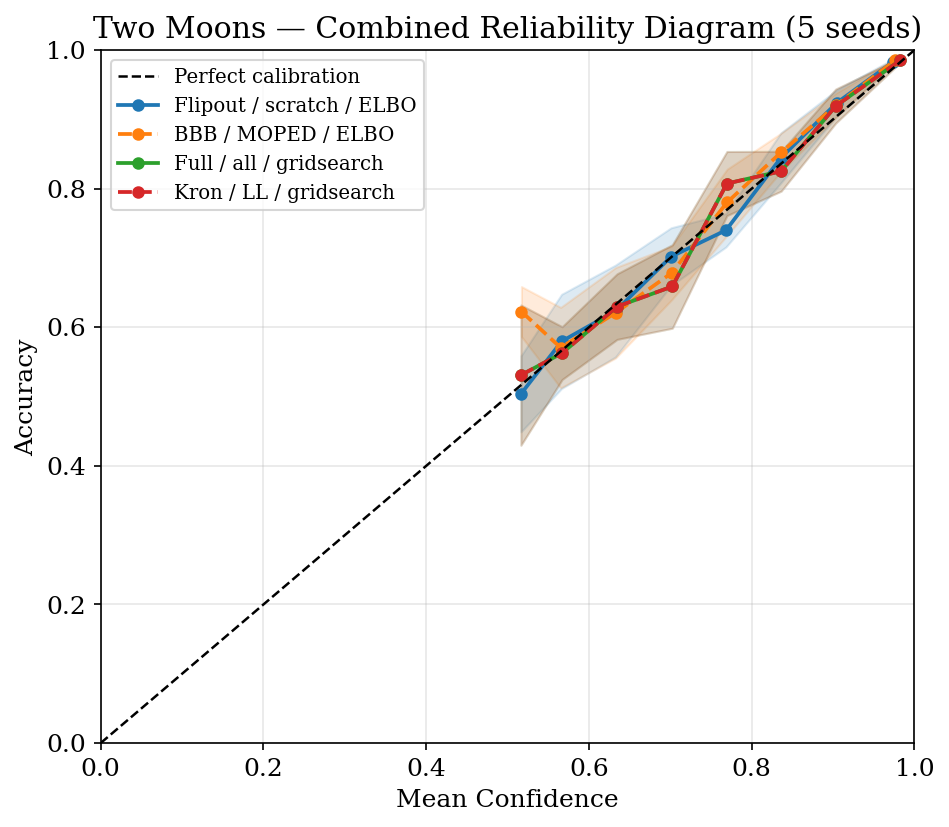
\includegraphics[width=0.75\linewidth]{5seed_two_moons_combined_reliability.png}
\caption{Combined 5-seed reliability diagram for the four best-tuned Two Moons variants.}
\label{fig:tm_reliability_combined}
\end{figure}

\begin{figure}[t]
\centering
\begin{subfigure}{\linewidth}
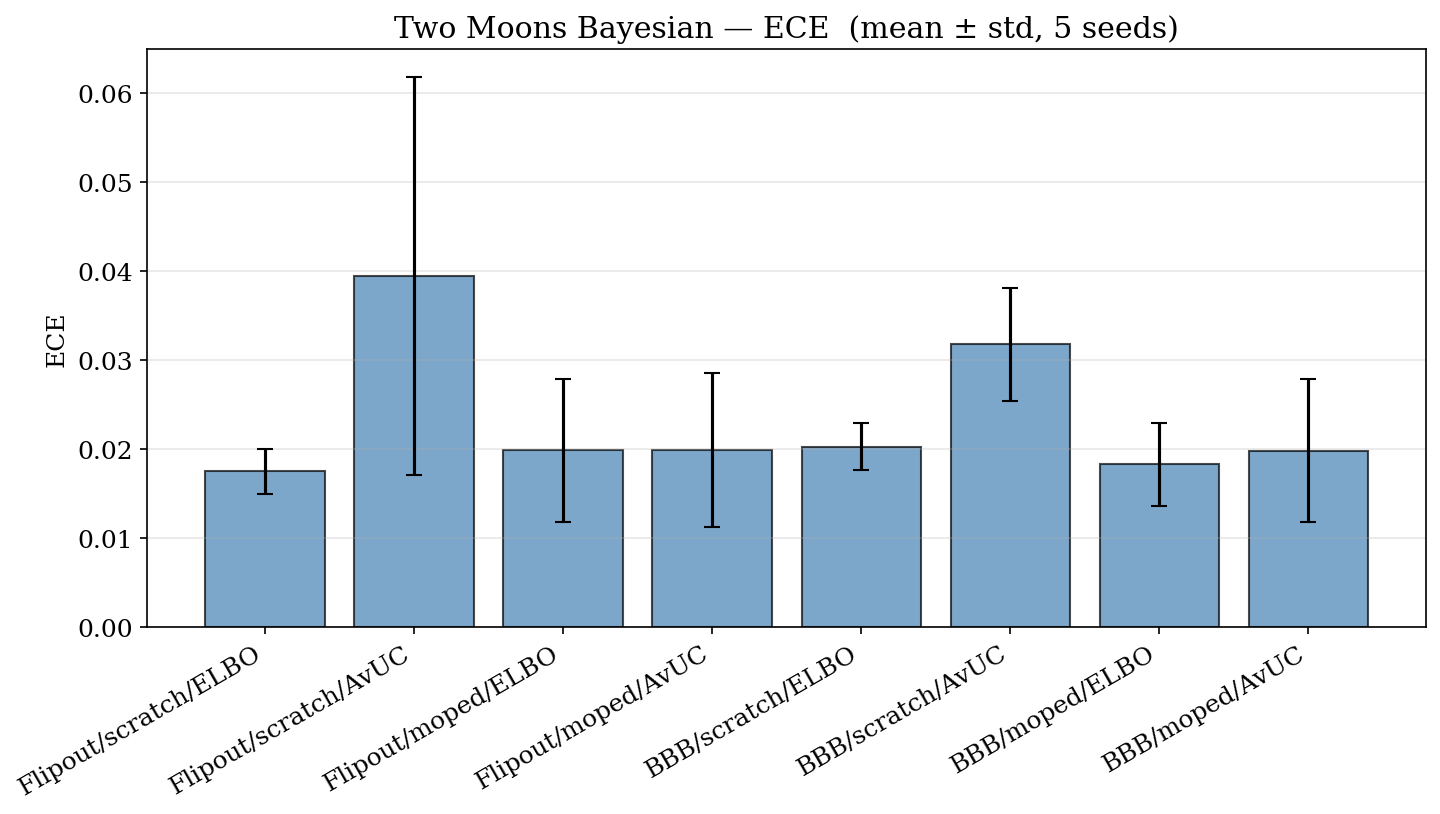
\includegraphics[width=\linewidth]{5seed_two_moons_bayesian_ece_bar.png}
\caption{\texttt{bayesian-torch}}
\end{subfigure}
\\[6pt]
\begin{subfigure}{\linewidth}
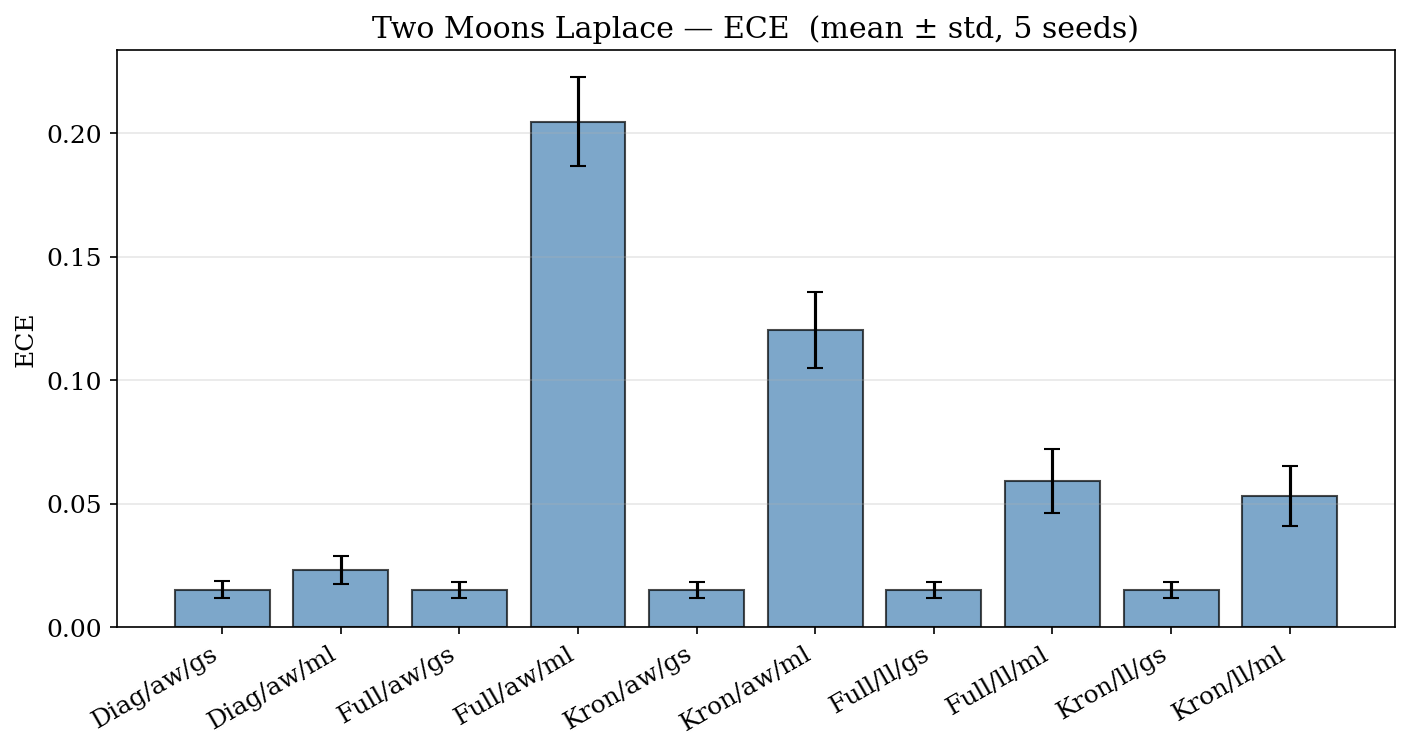
\includegraphics[width=\linewidth]{5seed_two_moons_laplace_ece_bar.png}
\caption{\texttt{laplace-torch}}
\end{subfigure}
\caption{5-seed ECE by variant, both methods.}
\label{fig:tm_ece_bars}
\end{figure}

\textbf{Epistemic uncertainty.} Figure~\ref{fig:tm_best_calib_heatmap} shows the
epistemic uncertainty map of the best-calibrated variant, Full / all weights / gridsearch.
Uncertainty is concentrated in a narrow band along the decision boundary and negligible over
the rest of the input space.

\begin{figure}[t]
\centering
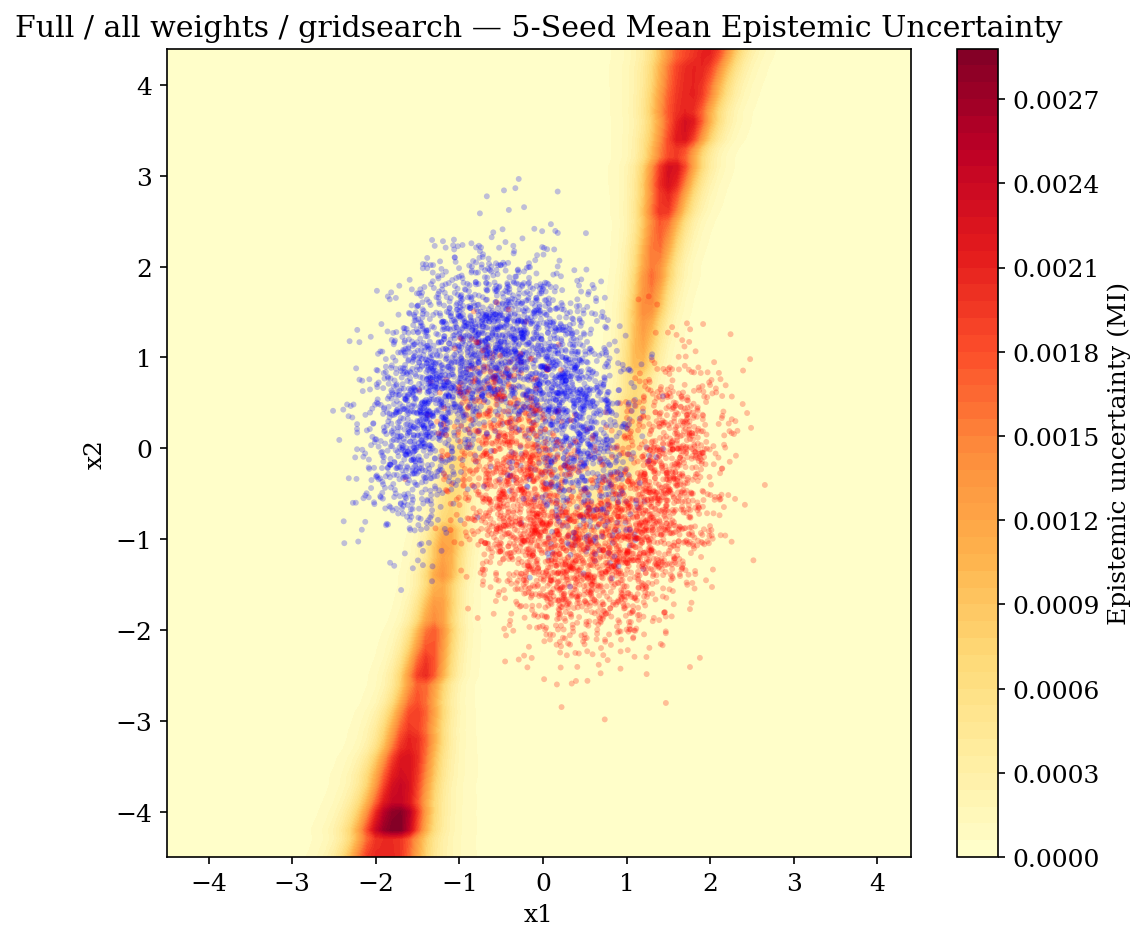
\includegraphics[width=0.6\linewidth]{5seed_two_moons_gridsearch_full_all_weights_epistemic_map.png}
\caption{5-seed mean epistemic uncertainty for the best-calibrated Two Moons variant, Full / all weights / gridsearch.}
\label{fig:tm_best_calib_heatmap}
\end{figure}

\textbf{Training time.} Figure~\ref{fig:tm_fit_time_bars} plots total time for every
variant of both methods; full timing is in Tables~\ref{tab:app:tm_bt}
and~\ref{tab:app:tm_la}. For \texttt{bayesian-torch}, AvUC loss costs an order of
magnitude more total time than ELBO, for both Flipout and BBB, MOPED or scratch. For
\texttt{laplace-torch}, full Hessian over all weights is by far the most expensive variant
(Total $\approx 1195\,\text{s}$, versus under $20\,\text{s}$ for every other variant);
diagonal and Kronecker-factored Hessians are similarly cheap regardless of tuning method. A
single shared MAP step ($9.4 \pm 1.6\,\text{s}$) is included in this total for all ten
\texttt{laplace-torch} variants and for \texttt{bayesian-torch}'s MOPED variants;
\texttt{bayesian-torch}'s scratch variants skip it.

\begin{figure}[t]
\centering
\begin{subfigure}{\linewidth}

\includegraphics[width=\linewidth]{5seed_two_moons_bayesian_total_time_bar.png}
\caption{\texttt{bayesian-torch}}
\end{subfigure}
\\[6pt]
\begin{subfigure}{\linewidth}

\includegraphics[width=\linewidth]{5seed_two_moons_laplace_total_time_bar.png}
\caption{\texttt{laplace-torch}}
\end{subfigure}
\caption{5-seed mean total time by variant, both methods.}
\label{fig:tm_fit_time_bars}
\end{figure}

\textbf{Inference time.} \texttt{laplace-torch}'s last-layer-subset variants infer
$11$-$260\times$ faster than all-weights variants ($0.44$-$1.92\,\text{ms}$ vs.\
$20.5$-$114.4\,\text{ms}$), regardless of Hessian structure or tuning method;
\texttt{bayesian-torch}'s variants show no comparable split, ranging from $2.1$ to
$31.4\,\text{ms}$ (Tables~\ref{tab:app:tm_bt} and~\ref{tab:app:tm_la}).

\subsection{Sinusoid}

This dataset uses the regression metrics (RMSE, NLL, regression calibration error) and the
additive-variance epistemic uncertainty of Section~\ref{sec:theory:unc_decomp}. Results on
the small library-provided sinusoid dataset (Section~\ref{sec:imp:sinusoid}) are reported
separately in Appendix~\ref{sec:app:sinusoid_small}. The following covers the larger
comparison dataset.

\textbf{Initialisation and tuning.} For \texttt{bayesian-torch}, MOPED initialisation is
worse than training from scratch on this dataset, for both Flipout and BBB: scratch is both
more accurate and better calibrated (Table~\ref{tab:app:sin_big_bt}). Scratch also
calibrates better than MOPED on the small Sinusoid dataset
(Appendix~\ref{sec:app:sinusoid_small}); Two Moons is the exception, where MOPED improves
calibration for three of the four Flipout/BBB pairs. For \texttt{laplace-torch}, RMSE is
identical across all variants (all share the same MAP mean); calibration error varies
little with Hessian structure, weight subset, or tuning method (range $0.327$-$0.347$,
Table~\ref{tab:app:sin_big_la}).

\textbf{Calibration.} Figure~\ref{fig:sin_big_cal_bars} plots calibration error for every
variant of both methods; full values are in Tables~\ref{tab:app:sin_big_bt}
and~\ref{tab:app:sin_big_la}. The best-calibrated \texttt{bayesian-torch} variant is BBB /
scratch; the best-calibrated \texttt{laplace-torch} variant is Kron / all weights / adam
loop, tied within noise with the other Kron variants. Figure~\ref{fig:sin_big_cal_combined}
overlays the calibration curves of \texttt{bayesian-torch}'s two best-calibrated variants
(Flipout / scratch, BBB / scratch) against \texttt{laplace-torch}'s Kron / all weights /
adam loop and Kron / last layer / adam loop variants.

\begin{figure}[t]
\centering
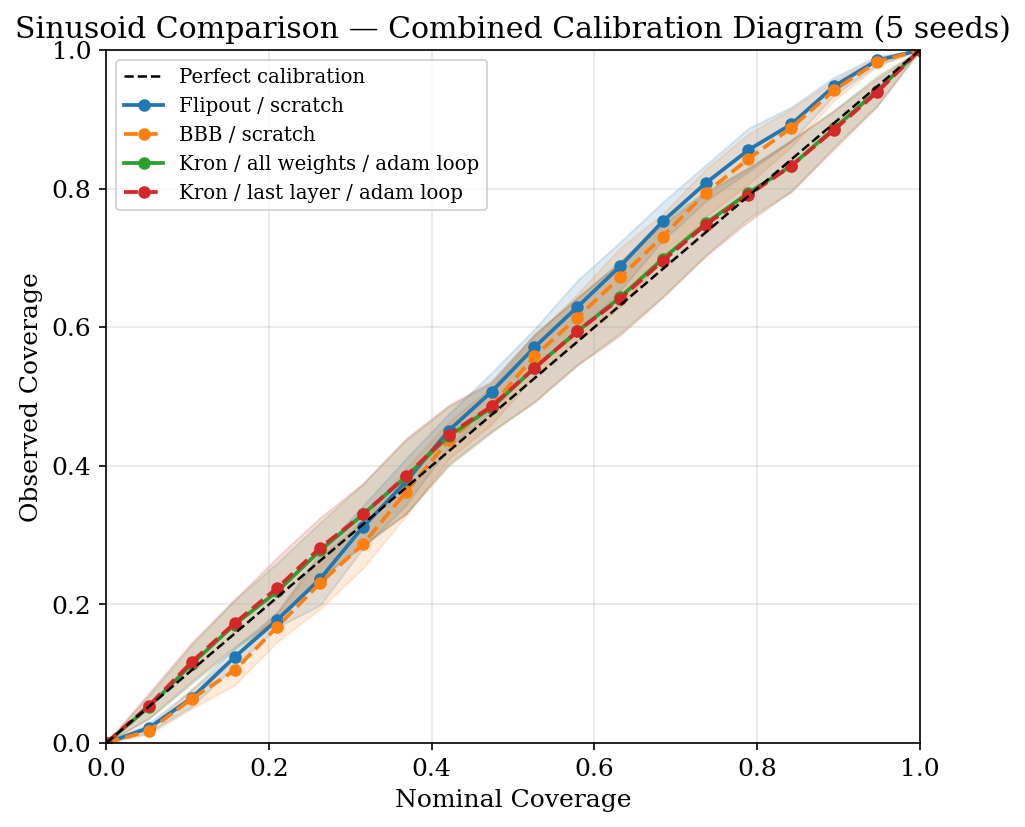
\includegraphics[width=0.75\linewidth]{5seed_sinusoid_comparison_combined_calibration.png}
\caption{Combined 5-seed calibration diagram for the Sinusoid comparison dataset.}
\label{fig:sin_big_cal_combined}
\end{figure}

\begin{figure}[t]
\centering
\begin{subfigure}{\linewidth}

\includegraphics[width=\linewidth]{5seed_sinusoid_comparison_bayesian_calibration_error_bar.png}
\caption{\texttt{bayesian-torch}}
\end{subfigure}
\\[6pt]
\begin{subfigure}{\linewidth}

\includegraphics[width=\linewidth]{5seed_sinusoid_comparison_laplace_calibration_error_bar.png}
\caption{\texttt{laplace-torch}}
\end{subfigure}
\caption{5-seed calibration error by variant, both methods, Sinusoid comparison dataset.}
\label{fig:sin_big_cal_bars}
\end{figure}

\textbf{Best-calibrated variant.} Figure~\ref{fig:sin_big_best_pred} shows the mean
prediction of the best-calibrated variant overall, Kron / all weights / adam loop, tracking
$\sin(x)$ closely inside the training range with a tight total-uncertainty band; its
epistemic uncertainty growth outside the training range is quantified below (Out-of-distribution
generalisation).

\begin{figure}[t]
\centering
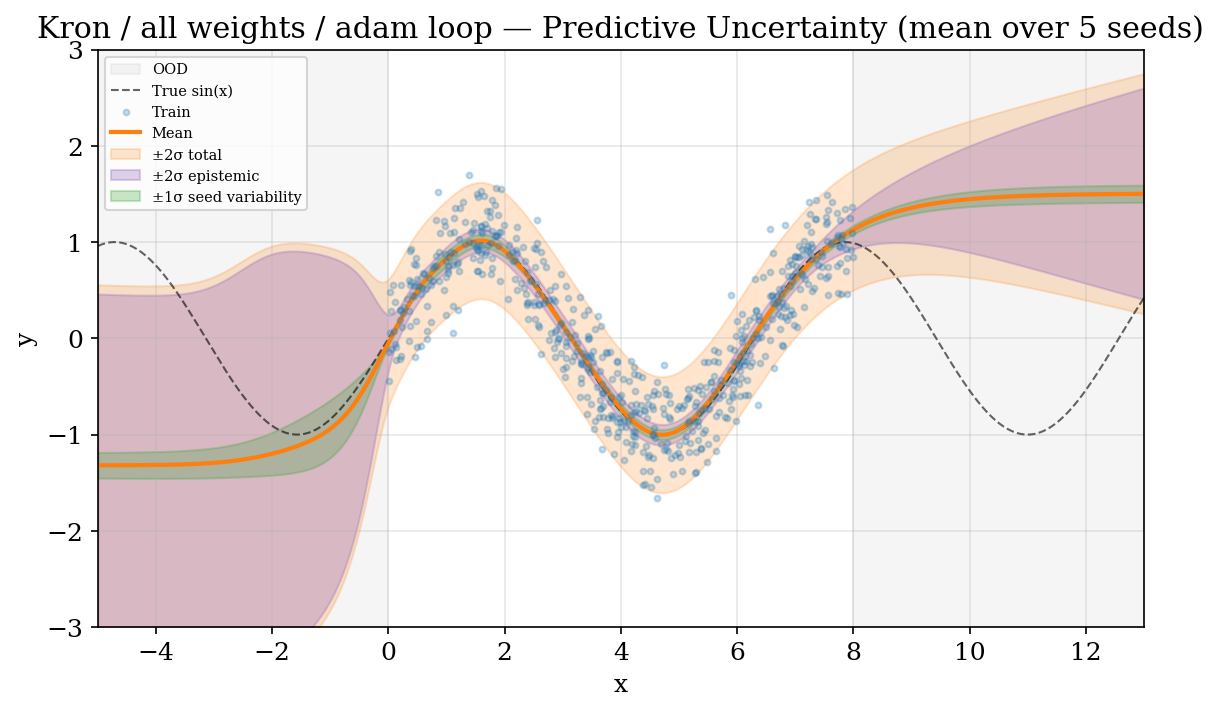
\includegraphics[width=0.75\linewidth]{sinusoid_comparison_kron_all_adam_loop_prediction.png}
\caption{5-seed mean prediction for the best-calibrated Sinusoid comparison-dataset variant, Kron / all weights / adam loop.}
\label{fig:sin_big_best_pred}
\end{figure}

\textbf{Training time.} Figure~\ref{fig:sin_big_fit_time_bars} plots total time for every
variant of both methods; full timing is in Tables~\ref{tab:app:sin_big_bt}
and~\ref{tab:app:sin_big_la}. For \texttt{bayesian-torch}, MOPED's own fit time is
lower than scratch's for both Flipout and BBB, but adding the shared MAP step flips the
ordering for Flipout: Flipout / moped has the highest total time of the four, despite being
worse calibrated; for BBB, MOPED remains cheaper even with the MAP step included. For
\texttt{laplace-torch}, the adam-loop-tuned Kron variants are the most expensive (tune time
$5.97$-$7.99\,\text{s}$, versus under $0.03\,\text{s}$ of fit time for both); full Hessian
over all weights (Total $15.05\,\text{s}$) is within $1\,\text{s}$ of the cheapest
gridsearch- and marglik-tuned variants ($14.18$-$14.19\,\text{s}$). A single shared MAP step
($13.7 \pm 0.7\,\text{s}$) is included in this total for all seven \texttt{laplace-torch}
variants and for \texttt{bayesian-torch}'s MOPED variants; \texttt{bayesian-torch}'s scratch
variants skip it.

\begin{figure}[t]
\centering
\begin{subfigure}{\linewidth}

\includegraphics[width=\linewidth]{5seed_sinusoid_comparison_bayesian_total_time_bar.png}
\caption{\texttt{bayesian-torch}}
\end{subfigure}
\\[6pt]
\begin{subfigure}{\linewidth}

\includegraphics[width=\linewidth]{5seed_sinusoid_comparison_laplace_total_time_bar.png}
\caption{\texttt{laplace-torch}}
\end{subfigure}
\caption{5-seed mean total time by variant, both methods, Sinusoid comparison dataset.}
\label{fig:sin_big_fit_time_bars}
\end{figure}

\textbf{Inference time.} \texttt{bayesian-torch}'s BBB infers roughly 35 times slower than
Flipout, for both scratch and MOPED initialisations. \texttt{laplace-torch}'s Kron / last
layer variants infer $3$-$4\times$ faster than Kron / all weights and Full / all weights
($0.35$-$0.40\,\text{ms}$ vs.\ $1.28$-$1.41\,\text{ms}$), regardless of tuning method
(Tables~\ref{tab:app:sin_big_bt} and~\ref{tab:app:sin_big_la}).

\textbf{Out-of-distribution generalisation.} Figure~\ref{fig:sin_epi_ratio_bars} plots
the epistemic ratio (OOD std / ID std) for every variant of both methods; full OOD metrics
are in Table~\ref{tab:app:sin_big_ood} (ID RMSE and NLL are in
Tables~\ref{tab:app:sin_big_bt} and~\ref{tab:app:sin_big_la}). Point-prediction RMSE
increases going OOD
for both methods: \texttt{bayesian-torch}'s OOD/ID RMSE ratio ranges from $1.71$ (BBB /
moped) to $8.17$ (Flipout / scratch); \texttt{laplace-torch}'s ratio is $5.12$ for every
variant (all share the same MAP mean). Epistemic uncertainty responds very differently
between methods: the three gridsearch-tuned \texttt{laplace-torch} variants (Kron / last
layer, Kron / all weights, Full / all weights) have the three highest epistemic ratios in
the table (Table~\ref{tab:app:sin_big_ood}); the remaining four \texttt{laplace-torch}
variants (marglik- and adam-loop-tuned) range from $7.3$ to $9.8$.
\texttt{bayesian-torch}'s scratch variants' epistemic ratios stay close to
$1$ ($1.26$ Flipout, $1.23$ BBB); its MOPED variants diverge: BBB falls below $1$ ($0.89$),
Flipout stays above it ($1.18$).

\begin{figure}[t]
\centering
\begin{subfigure}{\linewidth}

\includegraphics[width=\linewidth]{5seed_sinusoid_bayesian_epistemic_ratio_bar.png}
\caption{\texttt{bayesian-torch}}
\end{subfigure}
\\[6pt]
\begin{subfigure}{\linewidth}

\includegraphics[width=\linewidth]{5seed_sinusoid_laplace_epistemic_ratio_bar.png}
\caption{\texttt{laplace-torch}}
\end{subfigure}
\caption{5-seed OOD/ID epistemic ratio by variant, both methods.}
\label{fig:sin_epi_ratio_bars}
\end{figure}

\subsection{PovertyMap}

This dataset uses the same regression metrics and additive-variance epistemic uncertainty
(Section~\ref{sec:theory:unc_decomp}) as Sinusoid.

\textbf{Calibration.} Figure~\ref{fig:pm_cal_error_bar} plots ID and OOD calibration
error for both methods, mean $\pm$ std over 5 folds; full RMSE, NLL, and calibration error
values are in Table~\ref{tab:app:povertymap} and Figure~\ref{fig:pm_rmse_nll_bar} in the
Appendix. \texttt{bayesian-torch} has lower calibration error than \texttt{laplace-torch},
both ID ($1.35$ vs.\ $3.59$) and OOD ($26.1$ vs.\ $35.3$). Figure~\ref{fig:pm_calibration}
plots the calibration reliability diagram for both methods, ID and OOD.

\begin{figure}[t]
\centering
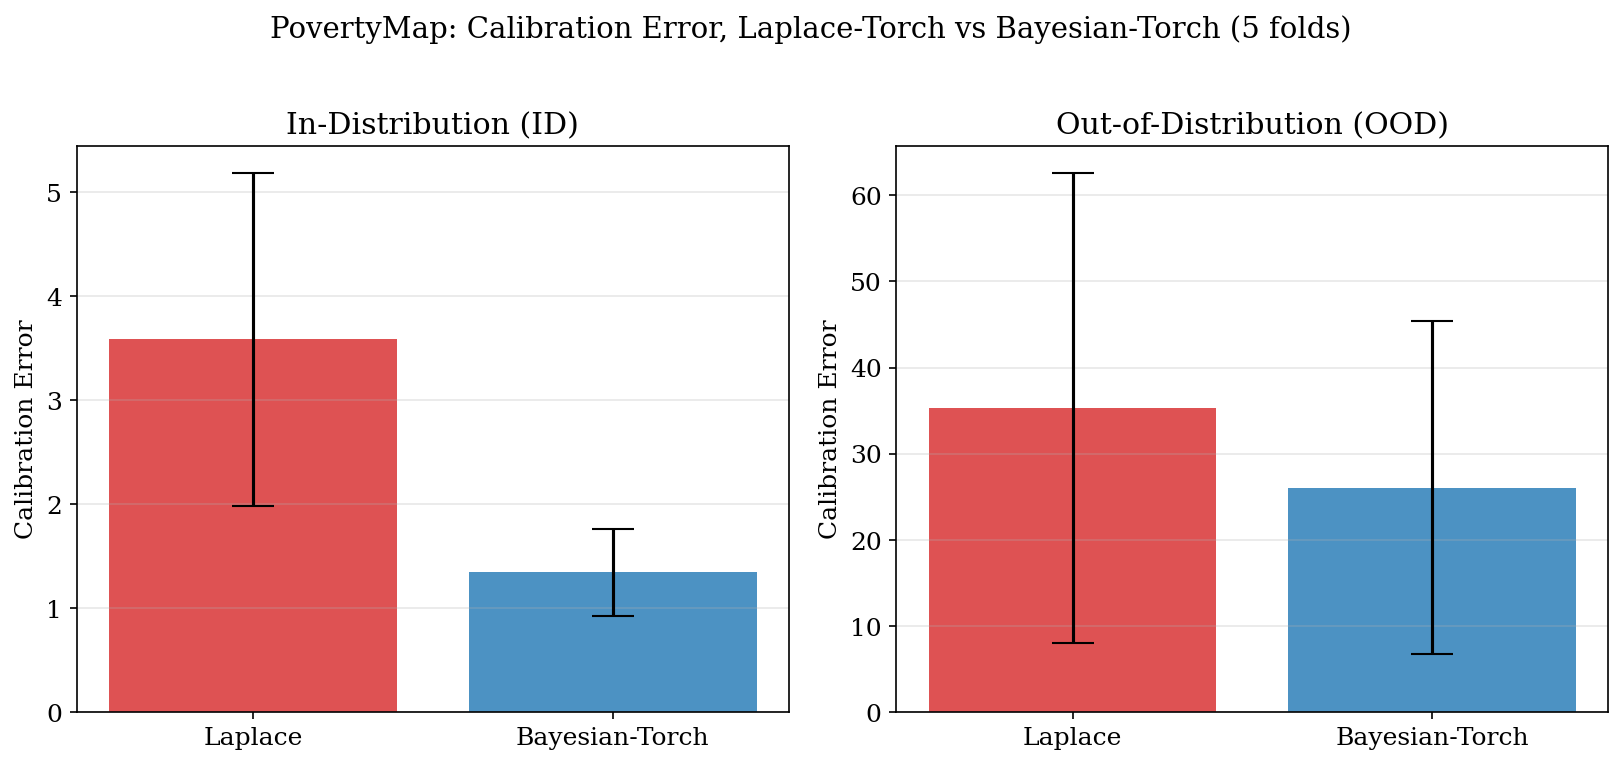
\includegraphics[width=\linewidth]{povertymap_cal_error_bar.png}
\caption{PovertyMap calibration error, ID and OOD, both methods (5 folds).}
\label{fig:pm_cal_error_bar}
\end{figure}

\begin{figure}[t]
\centering

\includegraphics[width=\linewidth]{povertymap_calibration_curves.png}
\caption{PovertyMap calibration reliability diagrams, ID and OOD, both methods (mean $\pm$ 1$\sigma$, 5 folds).}
\label{fig:pm_calibration}
\end{figure}

\textbf{Training time.} Figure~\ref{fig:pm_total_time_bar} plots total time for both
methods, mean $\pm$ std over 5 folds; full values are in Table~\ref{tab:app:povertymap}.
\texttt{bayesian-torch} takes $959.8 \pm 111.0\,\text{s}$ to train, roughly $22\times$
longer than \texttt{laplace-torch}'s $43.8 \pm 4.7\,\text{s}$.

\begin{figure}[t]
\centering
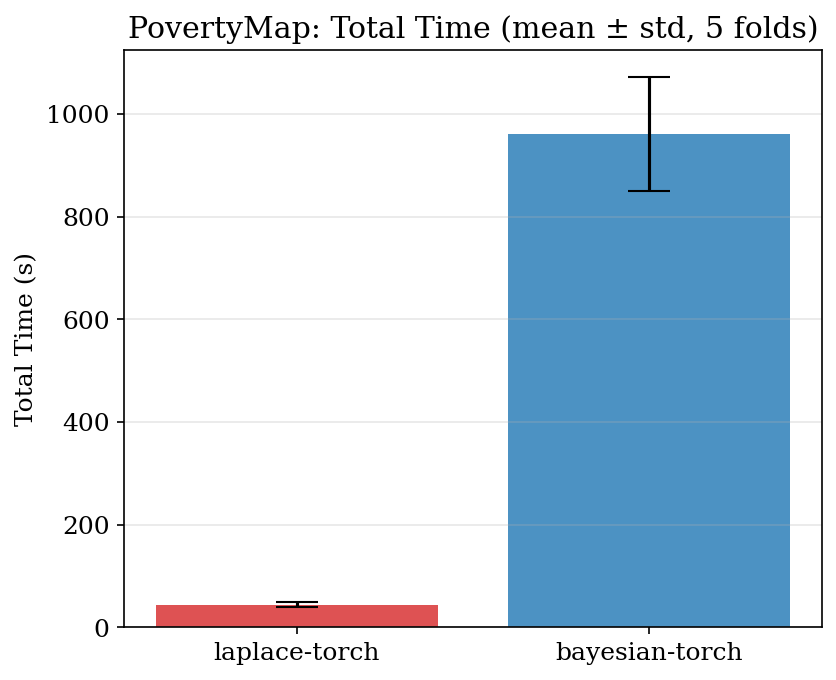
\includegraphics[width=0.6\linewidth]{povertymap_total_time_bar.png}
\caption{PovertyMap total time, both methods (5 folds).}
\label{fig:pm_total_time_bar}
\end{figure}

\textbf{Inference time.} \texttt{laplace-torch} infers faster than \texttt{bayesian-torch},
both ID ($2.3$ vs.\ $17.0\,\text{s}$) and OOD ($6.3$ vs.\ $61.2\,\text{s}$);
\texttt{bayesian-torch}'s PovertyMap variant loops over MC samples instead of tiling them
into a single forward pass like its other Flipout variants (Section~\ref{sec:imp})
(Table~\ref{tab:app:povertymap}).

\textbf{Variant ablations.}
\texttt{laplace-torch}'s NLL-gridsearched prior precision ($\approx 0.10$-$0.12$) and its
fixed headline value ($10.0$) stay within a few percent of each other on every metric, ID and
OOD. \texttt{bayesian-torch}'s three prior variants agree closely on RMSE and NLL, ID and
OOD, but spread further on calibration error. The headline configuration (fixed
$\tau=0.1$, prior precision scaled by $N$, matching \citet{daxberger2021laplace}'s released
training script) has the lowest OOD calibration error by a wide margin over both
$\tau$-annealing~\citep{osawa2019practical} and scaling the prior by batch size instead of
$N$ (\texttt{bayesian-torch}'s own default convention). On ID calibration error, though, the
batch-size-scaled default is instead the best of the three. Full per-variant metrics are in
the notebooks.

\section{Discussion}
\label{sec:discussion}

Two \texttt{laplace-torch} design choices trade off in opposite directions. Restricting the
Hessian to the last layer cuts inference cost dramatically ($11$-$260\times$ on Two Moons),
while the choice of tuning method dominates OOD behaviour. Marginal-likelihood and
gridsearch tuning give similar in-distribution calibration once Hessian and weight subset
are fixed (e.g.\ Kron/last calibration error $0.347$ vs.\ $0.345$, Kron/all $0.340$ vs.\
$0.333$ on Sinusoid-comparison, both within noise), but they diverge sharply out of
distribution: gridsearch reaches epistemic ratios of $77.1$ (Kron/last) and $47.6$
(Kron/all), versus marginal-likelihood's $7.29$ and $9.84$ for the same configurations.
Adam-loop's distinguishing feature is jointly tuning the aleatoric noise term alongside the
prior precision, rather than fixing it to the MAP residual as marginal-likelihood and
gridsearch both do; its ratios ($7.26$, $9.79$) track marginal-likelihood's, not
gridsearch's. The instability tracks the tuning method more than the weight subset.

Marginal-likelihood tuning is consistently faster than gridsearch and needs no held-out
validation split (e.g.\ $0.10\,\text{s}$ vs.\ $5.17\,\text{s}$ on Two Moons' Kron/all), at
the cost of worse NLL and ECE than gridsearch or adam-loop (Two Moons Full/all: ECE $0.205$
vs.\ $0.015$).

The epistemic-ratio picture does not resolve cleanly into a \texttt{laplace-torch}-wins
conclusion, however. The highest ratios come specifically from the gridsearch-tuned
variants already flagged above as less reliable, and carry standard deviations that often
exceed the mean itself; adam-loop's variants, better behaved by the criteria above, sit at
much lower ratios ($7$-$10\times$). \texttt{bayesian-torch}'s scratch variants grow only
about $1.2\times$ OOD, more modestly than even \texttt{laplace-torch}'s most stable
variants. Whether larger OOD growth reflects genuinely better awareness of distribution
shift or just a noisier estimate is not something the data here settles either way.

MOPED initialisation is not a universal improvement: it raises calibration and accuracy over
training from scratch on Two Moons and the small Sinusoid dataset, but reverses on the
larger Sinusoid comparison dataset, where scratch is both more accurate and better
calibrated. AvUC costs an order of magnitude more fit time than ELBO in every configuration
tested, and only improves calibration relative to its own from-scratch baseline, not
relative to ELBO once MOPED-initialised, making it hard to justify.

Whether \texttt{bayesian-torch} can match \texttt{laplace-torch} depends on the dataset. On
Two Moons the two are close, with \texttt{laplace-torch}'s best variant still slightly ahead
(ECE $0.0150$ vs.\ $0.0175$); on PovertyMap, the largest and most realistic experiment,
\texttt{bayesian-torch} wins outright on in-distribution RMSE, NLL, and calibration error,
and on OOD calibration error, though \texttt{laplace-torch} trains roughly $22\times$ faster
and infers $7$-$10\times$ faster and matches or beats \texttt{bayesian-torch} on OOD RMSE
and NLL; but on both Sinusoid datasets, \texttt{laplace-torch}'s best-calibrated variant
clearly beats \texttt{bayesian-torch}'s ($0.250$ vs.\ $1.026$ small, $0.327$ vs.\ $0.454$
comparison). This is not a general \texttt{bayesian-torch}-can-match-\texttt{laplace-torch}
story; it holds only on classification and the largest regression task. On inference time
\texttt{laplace-torch} generally wins, though only its last-layer variants do so on Two
Moons, where its all-weights variants are slower than \texttt{bayesian-torch}'s fastest
configuration.

\textbf{Limitations and threats to validity.} The experiments are limited to three
datasets, two of which are small and two of which are synthetic. There is a specific
concern with drawing conclusions from the Two Moons dataset alone, as there is no more
complex classification dataset to compare against. Moreover, there is no ID/OOD testing in
this experiment.

Testing all possible combinations of the variants possible in both libraries is rather
time-intensive, and so the experiments are limited to a subset of the possible
combinations. Ideally, all combinations could be tested to see what trends are consistent
across all combinations, and which are specific to a particular one. Hyperparameter tuning,
for example, is a very important part of the performance of some implementations, and there
is no set-in-stone strategy for finding the best hyperparameters.

There still remains the question of how well the OOD detection works in practice. This is
indeed discussed in \citet{daxberger2021laplace}, where results for \texttt{laplace-torch}
are favorable.

\textbf{Future work.} The experiments could be extended to include more datasets, and more
complex datasets, to see if the trends observed here hold in more realistic settings.
Additionally, further work could be done to explore the impact of different hyperparameter
tuning strategies on the performance of both libraries, and to investigate the
effectiveness of OOD detection in practice.

\section{Code Availability}
\label{sec:software}

\begin{itemize}[leftmargin=*]
	\item \texttt{bayesian-torch}:
	      \url{https://github.com/IntelLabs/bayesian-torch}
	\item \texttt{laplace-torch}:
	      \url{https://aleximmer.com/Laplace}
	\item \texttt{laplace-redux} (reproduces \citet{daxberger2021laplace}):
	      \url{https://github.com/runame/laplace-redux}
\end{itemize}

\appendix
\section{Appendix: Full Metric Tables and Visualizations}
\label{sec:app}

\subsection{Sinusoid: Small Library-Provided Dataset (150 samples)}
\label{sec:app:sinusoid_small}

Results below use the small, library-provided sinusoid dataset described in
Section~\ref{sec:imp:sinusoid} (150 train / 50 val / 250 ID test / 250 OOD test), rather
than the larger comparison dataset used for the main Sinusoid results, including the
out-of-distribution analysis below.

\begin{table}[H]
\centering
\resizebox{\linewidth}{!}{%
\begin{tabular}{llcccccc}
\toprule
Type & Init & RMSE & NLL & Cal. Error & Fit (s) & Inf (ms) & Total (s) \\
\midrule
Flipout & scratch & $0.596 \pm 0.087$ & $\bm{0.932 \pm 0.158}$ & $1.094 \pm 0.292$ & $160.26$ & $6.54$ & $160.26$ \\
Flipout & moped & $0.782 \pm 0.177$ & $1.472 \pm 0.177$ & $3.974 \pm 0.526$ & $1.71$ & $\bm{6.40}$ & $60.73$ \\
BBB & scratch & $0.697 \pm 0.024$ & $1.096 \pm 0.057$ & $\bm{1.026 \pm 0.447}$ & $120.22$ & $48.57$ & $120.22$ \\
BBB & moped & $\bm{0.590 \pm 0.031}$ & $1.568 \pm 0.052$ & $7.076 \pm 0.604$ & $\bm{0.46}$ & $49.42$ & $\bm{59.48}$ \\
\bottomrule
\end{tabular}}
\caption{\texttt{bayesian-torch} on Sinusoid (small dataset): 5-seed metrics and timing (mean $\pm$ std). Total time is fit time plus the shared MAP step ($59.0\,\text{s}$) for MOPED variants, fit time alone for scratch.}
\label{tab:app:sin_small_bt}
\end{table}

\begin{table}[H]
\centering
\resizebox{\linewidth}{!}{%
\begin{tabular}{lllcccccc}
\toprule
Hessian & Scope & Tuning & NLL & Cal. Error & Fit (s) & Tune (s) & Inf (ms) & Total (s) \\
\midrule
Diag & all & marglik & $0.323 \pm 0.011$ & $0.627 \pm 0.272$ & $0.17$ & $\bm{0.06}$ & $3.89$ & $\bm{59.25}$ \\
Diag & all & gridsearch & $0.312 \pm 0.026$ & $0.544 \pm 0.313$ & $0.18$ & $10.88$ & $3.49$ & $70.08$ \\
Kron & all & marglik & $0.276 \pm 0.024$ & $0.275 \pm 0.138$ & $0.51$ & $0.08$ & $1.42$ & $59.60$ \\
Kron & all & gridsearch & $0.274 \pm 0.025$ & $\bm{0.250 \pm 0.116}$ & $0.51$ & $14.55$ & $3.96$ & $74.08$ \\
Full & all & marglik & $0.276 \pm 0.029$ & $0.272 \pm 0.146$ & $5.40$ & $12.85$ & $2.66$ & $77.27$ \\
Full & all & gridsearch & $0.276 \pm 0.031$ & $0.274 \pm 0.154$ & $5.55$ & $19.44$ & $3.26$ & $84.01$ \\
Full & last layer & marglik & $0.278 \pm 0.032$ & $0.283 \pm 0.154$ & $0.13$ & $4.29$ & $2.06$ & $63.43$ \\
Full & last layer & gridsearch & $0.276 \pm 0.032$ & $0.278 \pm 0.155$ & $\bm{0.12}$ & $9.10$ & $1.63$ & $68.23$ \\
Kron & last layer & marglik & $0.278 \pm 0.031$ & $0.280 \pm 0.152$ & $0.23$ & $0.07$ & $2.40$ & $59.32$ \\
Kron & last layer & gridsearch & $\bm{0.273 \pm 0.029}$ & $0.259 \pm 0.139$ & $0.23$ & $2.07$ & $\bm{0.35}$ & $61.31$ \\
Kron & all & adam loop & $0.276 \pm 0.025$ & $0.276 \pm 0.140$ & $0.47$ & $0.88$ & $4.03$ & $60.36$ \\
Kron & last layer & adam loop & $0.278 \pm 0.032$ & $0.284 \pm 0.155$ & $0.22$ & $0.59$ & $1.06$ & $59.83$ \\
\bottomrule
\end{tabular}}
\caption{\texttt{laplace-torch} on Sinusoid (small dataset): 5-seed metrics and timing (mean $\pm$ std). RMSE is identical across all variants ($0.317 \pm 0.009$), since it depends only on the shared MAP mean. Total time is the shared MAP step ($59.0\,\text{s}$) plus fit plus tune time, since every variant requires the MAP step.}
\label{tab:app:sin_small_la}
\end{table}

\textbf{Tuning.} For \texttt{bayesian-torch}, scratch initialisation reaches
$3.6$-$6.9\times$ better calibration error than MOPED, for both Flipout and BBB; RMSE is not
correspondingly worse for MOPED (Table~\ref{tab:app:sin_small_bt}). For
\texttt{laplace-torch}, RMSE is identical across every variant, since it depends only on the
shared MAP mean; calibration error varies with posterior choice, with Kron and Full Hessians
calibrating roughly $2\times$ better than Diagonal (Table~\ref{tab:app:sin_small_la}).
Marglik tuning is comparable to or slightly worse than gridsearch or the Adam-loop.

\textbf{Calibration.} Figure~\ref{fig:sin_cal_bars} plots calibration error for every
variant of both methods; full values are in Tables~\ref{tab:app:sin_small_bt}
and~\ref{tab:app:sin_small_la}. The best-calibrated \texttt{bayesian-torch} variant is BBB /
scratch; the best-calibrated \texttt{laplace-torch} variant is Kron / all weights /
gridsearch. Figure~\ref{fig:sin_cal_combined} overlays the calibration curves of
\texttt{bayesian-torch}'s two best-calibrated variants (Flipout / scratch, BBB / scratch)
against \texttt{laplace-torch}'s single best (Kron / all weights / gridsearch): both
\texttt{bayesian-torch} curves show an S-shape; Kron / all weights / gridsearch tracks the
diagonal closely across the full range.

\begin{figure}[t]
\centering
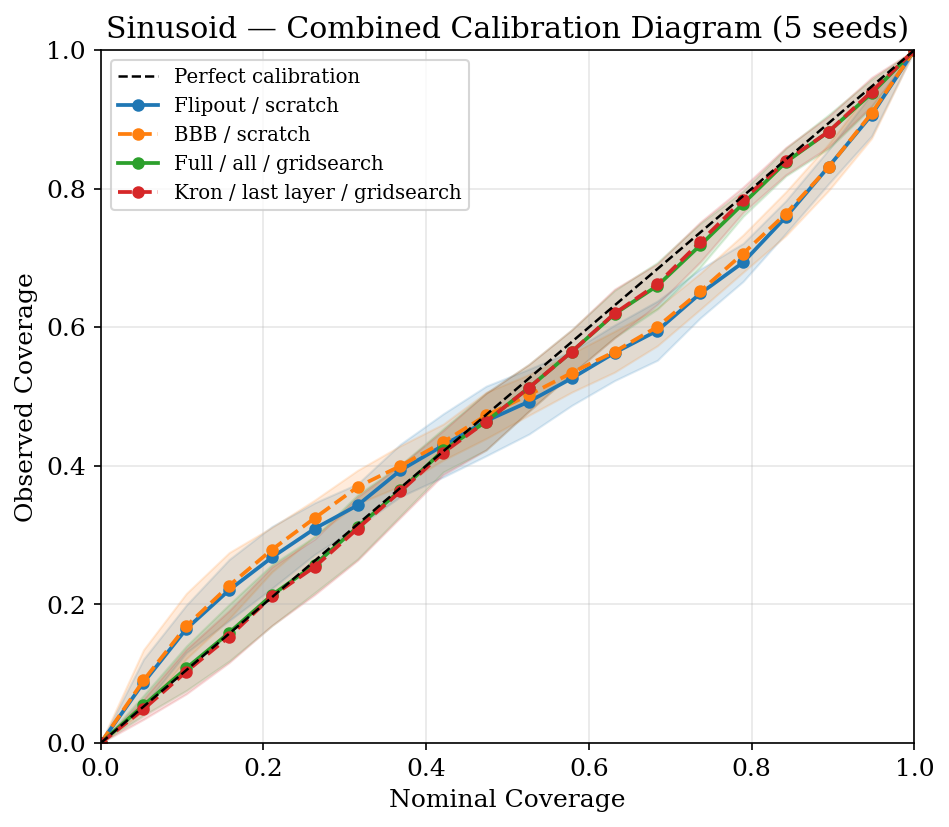
\includegraphics[width=0.75\linewidth]{5seed_sinusoid_combined_calibration.png}
\caption{Combined 5-seed calibration diagram for the best-calibrated Sinusoid variants.}
\label{fig:sin_cal_combined}
\end{figure}

\begin{figure}[t]
\centering
\begin{subfigure}{\linewidth}

\includegraphics[width=\linewidth]{5seed_sinusoid_bayesian_calibration_error_bar.png}
\caption{\texttt{bayesian-torch}}
\end{subfigure}
\\[6pt]
\begin{subfigure}{\linewidth}

\includegraphics[width=\linewidth]{5seed_sinusoid_laplace_calibration_error_bar.png}
\caption{\texttt{laplace-torch}}
\end{subfigure}
\caption{5-seed calibration error by variant, both methods.}
\label{fig:sin_cal_bars}
\end{figure}

\textbf{Best-calibrated variant.} Figure~\ref{fig:sin_best_pred} shows the mean prediction
of the best-calibrated variant overall, Kron / all weights / gridsearch, tracking $\sin(x)$
closely inside the training range $[0,8]$ with a tight total-uncertainty band; its epistemic
uncertainty growth outside the training range is quantified below (Out-of-distribution
generalisation).

\begin{figure}[t]
\centering

\includegraphics[width=0.75\linewidth]{5seed_sinusoid_kron_all_gridsearch_prediction.png}
\caption{5-seed mean prediction for the best-calibrated Sinusoid variant, Kron / all weights / gridsearch.}
\label{fig:sin_best_pred}
\end{figure}

\textbf{Training time.} Figure~\ref{fig:sin_fit_time_bars} plots total time for every
variant of both methods; full timing is in Tables~\ref{tab:app:sin_small_bt}
and~\ref{tab:app:sin_small_la}. For \texttt{bayesian-torch}, MOPED roughly halves
total time relative to scratch, for both Flipout and BBB. For \texttt{laplace-torch}, full
Hessian over all weights is the most expensive variant (Total $\approx 84\,\text{s}$ here,
versus $\approx 1195\,\text{s}$ on Two Moons); the cheapest variants add well under a second
of fit and tune time on top of the shared MAP step.

\begin{figure}[t]
\centering
\begin{subfigure}{\linewidth}

\includegraphics[width=\linewidth]{5seed_sinusoid_bayesian_total_time_bar.png}
\caption{\texttt{bayesian-torch}}
\end{subfigure}
\\[6pt]
\begin{subfigure}{\linewidth}

\includegraphics[width=\linewidth]{5seed_sinusoid_laplace_total_time_bar.png}
\caption{\texttt{laplace-torch}}
\end{subfigure}
\caption{5-seed mean total time by variant, both methods.}
\label{fig:sin_fit_time_bars}
\end{figure}

\textbf{Inference time.} \texttt{laplace-torch} infers faster than \texttt{bayesian-torch}
for every variant, though both methods stay under a tenth of a second
(Tables~\ref{tab:app:sin_small_bt} and~\ref{tab:app:sin_small_la}).

\textbf{Out-of-distribution generalisation.} Figure~\ref{fig:sin_small_epi_ratio_bars}
plots the epistemic ratio (OOD std / ID std) for every variant of both methods; full OOD
metrics are in Table~\ref{tab:app:sin_small_ood} (ID RMSE and NLL are in
Tables~\ref{tab:app:sin_small_bt} and~\ref{tab:app:sin_small_la}). As on the comparison dataset
(Section~\ref{sec:results}), every \texttt{laplace-torch} variant's epistemic uncertainty
grows going OOD; Kron / last layer / gridsearch (ratio $60.8$), Kron / all weights /
gridsearch ($50.0$), and Full / all weights / marglik ($39.6$) grow the most, Diagonal the
least ($1.4$-$1.8$). \texttt{bayesian-torch}'s scratch variants grow only modestly
($1.23$-$1.27$), and its MOPED variants' epistemic uncertainty shrinks going OOD
($0.79$-$0.92$).

\begin{figure}[t]
\centering
\begin{subfigure}{\linewidth}

\includegraphics[width=\linewidth]{5seed_sinusoid_small_bayesian_epistemic_ratio_bar.png}
\caption{\texttt{bayesian-torch}}
\end{subfigure}
\\[6pt]
\begin{subfigure}{\linewidth}

\includegraphics[width=\linewidth]{5seed_sinusoid_small_laplace_epistemic_ratio_bar.png}
\caption{\texttt{laplace-torch}}
\end{subfigure}
\caption{5-seed OOD/ID epistemic ratio by variant, both methods, small Sinusoid dataset.}
\label{fig:sin_small_epi_ratio_bars}
\end{figure}

\begin{table*}[!t]
\centering
\scriptsize
\resizebox{\textwidth}{!}{%
\begin{tabular}{llccccc}
\toprule
Method & Variant & OOD RMSE & OOD NLL & ID Epi & OOD Epi & Epi Ratio \\
\midrule
BT & Flipout / scratch & $1.535 \pm 0.158$ & $4.837 \pm 0.979$ & $0.183 \pm 0.014$ & $0.225 \pm 0.014$ & $1.228 \pm 0.064$ \\
BT & Flipout / moped & $1.468 \pm 0.402$ & $1.850 \pm 0.291$ & $1.392 \pm 0.289$ & $1.094 \pm 0.248$ & $\bm{0.785 \pm 0.099}$ \\
BT & BBB / scratch & $1.177 \pm 0.095$ & $2.466 \pm 0.369$ & $0.161 \pm 0.011$ & $\bm{0.204 \pm 0.014}$ & $1.266 \pm 0.025$ \\
BT & BBB / moped & $\bm{1.149 \pm 0.069}$ & $\bm{1.680 \pm 0.049}$ & $1.700 \pm 0.102$ & $1.565 \pm 0.127$ & $0.920 \pm 0.046$ \\
Laplace & Diag / all / marglik & $1.725 \pm 0.211$ & $8.807 \pm 2.084$ & $0.269 \pm 0.015$ & $0.369 \pm 0.078$ & $1.378 \pm 0.297$ \\
Laplace & Diag / all / gridsearch & $1.725 \pm 0.211$ & $9.978 \pm 2.857$ & $0.234 \pm 0.077$ & $0.472 \pm 0.282$ & $1.836 \pm 0.799$ \\
Laplace & Kron / all / marglik & $1.725 \pm 0.211$ & $2.641 \pm 0.884$ & $0.120 \pm 0.008$ & $1.970 \pm 0.376$ & $16.571 \pm 3.679$ \\
Laplace & Kron / all / gridsearch & $1.725 \pm 0.211$ & $7.028 \pm 5.002$ & $0.117 \pm 0.044$ & $7.980 \pm 9.069$ & $49.977 \pm 52.155$ \\
Laplace & Full / all / marglik & $1.725 \pm 0.211$ & $2.309 \pm 0.134$ & $0.085 \pm 0.007$ & $3.330 \pm 0.427$ & $39.587 \pm 6.311$ \\
Laplace & Full / all / gridsearch & $1.725 \pm 0.211$ & $8.754 \pm 5.432$ & $0.064 \pm 0.023$ & $1.835 \pm 2.283$ & $20.855 \pm 22.602$ \\
Laplace & Full / last layer / marglik & $1.725 \pm 0.211$ & $7.486 \pm 2.772$ & $0.064 \pm 0.005$ & $0.840 \pm 0.092$ & $13.252 \pm 1.872$ \\
Laplace & Full / last layer / gridsearch & $1.725 \pm 0.211$ & $10.351 \pm 6.047$ & $\bm{0.056 \pm 0.018}$ & $1.869 \pm 2.148$ & $25.169 \pm 26.321$ \\
Laplace & Kron / last layer / marglik & $1.725 \pm 0.211$ & $7.708 \pm 2.828$ & $0.068 \pm 0.005$ & $0.696 \pm 0.093$ & $10.267 \pm 1.753$ \\
Laplace & Kron / last layer / gridsearch & $1.725 \pm 0.211$ & $8.011 \pm 4.780$ & $0.075 \pm 0.027$ & $6.161 \pm 6.729$ & $60.798 \pm 61.883$ \\
Laplace & Kron / all / adam loop & $1.725 \pm 0.211$ & $2.647 \pm 0.892$ & $0.120 \pm 0.008$ & $1.966 \pm 0.377$ & $16.588 \pm 3.695$ \\
Laplace & Kron / last layer / adam loop & $1.725 \pm 0.211$ & $7.742 \pm 2.844$ & $0.068 \pm 0.005$ & $0.695 \pm 0.093$ & $10.290 \pm 1.757$ \\
\bottomrule
\end{tabular}}
\caption{Both methods on Sinusoid (small dataset), OOD metrics: 5-seed metrics (mean $\pm$ std). ID RMSE and NLL are in Tables~\ref{tab:app:sin_small_bt} and~\ref{tab:app:sin_small_la}.}
\label{tab:app:sin_small_ood}
\end{table*}

\subsection{Two Moons: Full Results}

Full metric and timing tables for every Two Moons variant of both methods are below, along
with accuracy and NLL bar charts not shown in the main Results (Section~\ref{sec:results}).

\begin{table*}[!t]
\centering
\resizebox{\linewidth}{!}{%
\begin{tabular}{lllccccccc}
\toprule
Type & Init & Loss & Acc & NLL & BS & ECE & Fit (s) & Inf (ms) & Total (s) \\
\midrule
Flipout & scratch & ELBO & $0.9145 \pm 0.0101$ & $0.2200 \pm 0.0188$ & $0.0643 \pm 0.0064$ & $\bm{0.0175 \pm 0.0026}$ & $39.79$ & $31.39$ & $39.79$ \\
Flipout & scratch & AvUC & $0.9023 \pm 0.0105$ & $0.2497 \pm 0.0152$ & $0.0734 \pm 0.0053$ & $0.0394 \pm 0.0224$ & $662.95$ & $2.51$ & $662.95$ \\
Flipout & moped & ELBO & $0.9150 \pm 0.0064$ & $0.2138 \pm 0.0147$ & $0.0628 \pm 0.0051$ & $0.0198 \pm 0.0080$ & $26.66$ & $2.53$ & $36.07$ \\
Flipout & moped & AvUC & $0.9106 \pm 0.0055$ & $0.2205 \pm 0.0135$ & $0.0652 \pm 0.0043$ & $0.0199 \pm 0.0087$ & $351.12$ & $\bm{2.08}$ & $360.53$ \\
BBB & scratch & ELBO & $0.9108 \pm 0.0093$ & $0.2228 \pm 0.0191$ & $0.0653 \pm 0.0065$ & $0.0202 \pm 0.0026$ & $29.95$ & $28.92$ & $\bm{29.95}$ \\
BBB & scratch & AvUC & $0.9080 \pm 0.0096$ & $0.2330 \pm 0.0150$ & $0.0680 \pm 0.0053$ & $0.0317 \pm 0.0063$ & $672.14$ & $25.98$ & $672.14$ \\
BBB & moped & ELBO & $\bm{0.9152 \pm 0.0072}$ & $\bm{0.2121 \pm 0.0141}$ & $\bm{0.0625 \pm 0.0048}$ & $0.0182 \pm 0.0047$ & $\bm{21.10}$ & $26.33$ & $30.52$ \\
BBB & moped & AvUC & $0.9137 \pm 0.0067$ & $0.2143 \pm 0.0147$ & $0.0631 \pm 0.0050$ & $0.0198 \pm 0.0081$ & $370.60$ & $25.83$ & $380.02$ \\
\bottomrule
\end{tabular}}
\caption{\texttt{bayesian-torch} on Two Moons: 5-seed metrics and timing (mean $\pm$ std). Total time is fit time plus the shared MAP step ($9.4\,\text{s}$) for MOPED variants, fit time alone for scratch.}
\label{tab:app:tm_bt}
\end{table*}

\begin{table*}[!t]
\centering
\resizebox{\linewidth}{!}{%
\begin{tabular}{lllccccccc}
\toprule
Hessian & Scope & Tuning & NLL & BS & ECE & Fit (s) & Tune (s) & Inf (ms) & Total (s) \\
\midrule
Diag & all weights & gridsearch & $0.2065 \pm 0.0143$ & $0.0616 \pm 0.0047$ & $0.0152 \pm 0.0033$ & $0.23$ & $4.34$ & $114.41$ & $13.99$ \\
Diag & all weights & marglik & $0.2102 \pm 0.0124$ & $0.0620 \pm 0.0044$ & $0.0232 \pm 0.0056$ & $\bm{0.23}$ & $\bm{0.07}$ & $20.54$ & $\bm{9.71}$ \\
Full & all weights & gridsearch & $0.2065 \pm 0.0143$ & $0.0616 \pm 0.0047$ & $\bm{0.0150 \pm 0.0033}$ & $1180.70$ & $8.41$ & $71.64$ & $1198.53$ \\
Full & all weights & marglik & $0.3808 \pm 0.0189$ & $0.1069 \pm 0.0072$ & $0.2048 \pm 0.0180$ & $1181.83$ & $1.87$ & $31.88$ & $1193.11$ \\
Kron & all weights & gridsearch & $0.2065 \pm 0.0143$ & $0.0616 \pm 0.0047$ & $0.0150 \pm 0.0033$ & $0.53$ & $5.17$ & $26.37$ & $15.12$ \\
Kron & all weights & marglik & $0.2889 \pm 0.0141$ & $0.0777 \pm 0.0046$ & $0.1204 \pm 0.0153$ & $0.52$ & $0.10$ & $21.28$ & $10.03$ \\
Full & last layer & gridsearch & $0.2065 \pm 0.0143$ & $0.0616 \pm 0.0047$ & $0.0151 \pm 0.0033$ & $8.25$ & $1.50$ & $1.92$ & $19.16$ \\
Full & last layer & marglik & $0.2346 \pm 0.0110$ & $0.0657 \pm 0.0038$ & $0.0591 \pm 0.0129$ & $8.32$ & $0.09$ & $0.56$ & $17.82$ \\
Kron & last layer & gridsearch & $\bm{0.2065 \pm 0.0143}$ & $\bm{0.0616 \pm 0.0047}$ & $0.0150 \pm 0.0033$ & $0.42$ & $1.89$ & $0.45$ & $11.72$ \\
Kron & last layer & marglik & $0.2294 \pm 0.0108$ & $0.0648 \pm 0.0038$ & $0.0531 \pm 0.0122$ & $0.43$ & $0.08$ & $\bm{0.44}$ & $9.92$ \\
\bottomrule
\end{tabular}}
\caption{\texttt{laplace-torch} on Two Moons: 5-seed metrics and timing (mean $\pm$ std). Accuracy is identical across all variants ($0.9154 \pm 0.0056$), since it depends only on the shared MAP mean. Total time is the shared MAP step ($9.4\,\text{s}$) plus fit plus tune time, since every variant requires the MAP step.}
\label{tab:app:tm_la}
\end{table*}

\begin{figure}[t]
\centering
\begin{subfigure}{\linewidth}
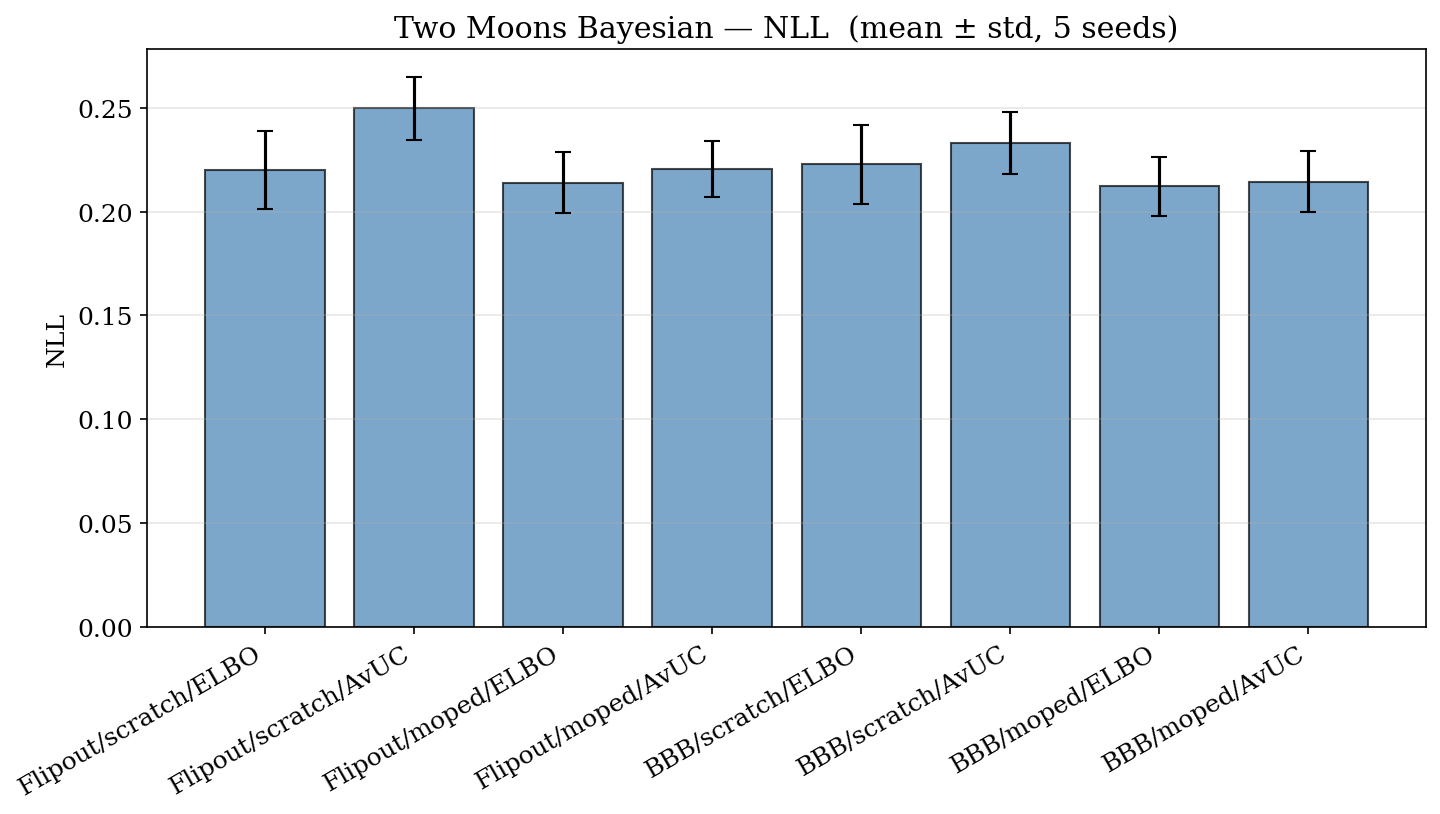
\includegraphics[width=\linewidth]{5seed_two_moons_bayesian_nll_bar.png}
\caption{\texttt{bayesian-torch}}
\end{subfigure}
\\[6pt]
\begin{subfigure}{\linewidth}

\includegraphics[width=\linewidth]{5seed_two_moons_laplace_nll_bar.png}
\caption{\texttt{laplace-torch}}
\end{subfigure}
\caption{5-seed NLL by variant, both methods.}
\label{fig:app:tm_nll_bars}
\end{figure}

\textbf{Accuracy and NLL.} Figure~\ref{fig:app:tm_nll_bars} plots NLL for every variant of
both methods; full values, including accuracy, are in Tables~\ref{tab:app:tm_bt}
and~\ref{tab:app:tm_la}. \texttt{bayesian-torch}'s accuracy ranges
$0.9023$-$0.9152$ across variants; \texttt{laplace-torch}'s accuracy is $0.9154 \pm 0.0056$
for every variant. NLL ranges $0.2121$-$0.2497$ for \texttt{bayesian-torch} and
$0.2065$-$0.3808$ for \texttt{laplace-torch}.

\subsection{Sinusoid: Comparison Dataset (600/200/200/200 split), ID vs OOD}
\label{sec:app:sinusoid_big}

\begin{table}[H]
\centering
\resizebox{\linewidth}{!}{%
\begin{tabular}{llcccccc}
\toprule
Type & Init & RMSE & NLL & Cal. Error & Fit (s) & Inf (ms) & Total (s) \\
\midrule
Flipout & scratch & $0.320 \pm 0.006$ & $0.319 \pm 0.015$ & $0.520 \pm 0.334$ & $12.97$ & $0.25$ & $\bm{12.97}$ \\
Flipout & moped & $0.398 \pm 0.106$ & $0.589 \pm 0.324$ & $1.203 \pm 1.321$ & $8.37$ & $\bm{0.25}$ & $22.04$ \\
BBB & scratch & $\bm{0.316 \pm 0.005}$ & $\bm{0.310 \pm 0.010}$ & $\bm{0.454 \pm 0.318}$ & $20.67$ & $8.63$ & $20.67$ \\
BBB & moped & $0.604 \pm 0.018$ & $1.339 \pm 0.104$ & $3.456 \pm 1.049$ & $\bm{2.55}$ & $8.64$ & $16.22$ \\
\bottomrule
\end{tabular}}
\caption{\texttt{bayesian-torch} on Sinusoid (comparison dataset), in-distribution: 5-seed metrics and timing (mean $\pm$ std). Total time is fit time plus the shared MAP step ($13.7\,\text{s}$) for MOPED variants, fit time alone for scratch.}
\label{tab:app:sin_big_bt}
\end{table}

\begin{table}[H]
\centering
\resizebox{\linewidth}{!}{%
\begin{tabular}{lllcccccc}
\toprule
Hessian & Scope & Tuning & NLL & Cal. Error & Fit (s) & Tune (s) & Inf (ms) & Total (s) \\
\midrule
Kron & last layer & marglik & $0.247 \pm 0.031$ & $0.345 \pm 0.251$ & $0.09$ & $\bm{0.42}$ & $0.40$ & $\bm{14.18}$ \\
Kron & last layer & gridsearch & $0.247 \pm 0.031$ & $0.347 \pm 0.253$ & $\bm{0.02}$ & $0.50$ & $\bm{0.35}$ & $14.19$ \\
Kron & last layer & adam loop & $0.246 \pm 0.030$ & $0.337 \pm 0.252$ & $0.02$ & $5.97$ & $0.35$ & $19.66$ \\
Kron & all weights & marglik & $0.246 \pm 0.031$ & $0.333 \pm 0.242$ & $0.03$ & $0.65$ & $1.39$ & $14.35$ \\
Kron & all weights & gridsearch & $\bm{0.245 \pm 0.031}$ & $0.340 \pm 0.247$ & $0.03$ & $0.87$ & $1.41$ & $14.57$ \\
Kron & all weights & adam loop & $0.246 \pm 0.030$ & $\bm{0.327 \pm 0.239}$ & $0.03$ & $7.99$ & $1.28$ & $21.68$ \\
Full & all weights & gridsearch & $0.247 \pm 0.031$ & $0.346 \pm 0.256$ & $0.88$ & $0.50$ & $1.31$ & $15.05$ \\
\bottomrule
\end{tabular}}
\caption{\texttt{laplace-torch} on Sinusoid (comparison dataset), in-distribution: 5-seed metrics and timing (mean $\pm$ std). RMSE is identical across all variants ($0.309 \pm 0.009$), since it depends only on the shared MAP mean. Total time is the shared MAP step ($13.7\,\text{s}$) plus fit plus tune time, since every variant requires the MAP step.}
\label{tab:app:sin_big_la}
\end{table}

\begin{table*}[!t]
\centering
\scriptsize
\resizebox{\textwidth}{!}{%
\begin{tabular}{llccccc}
\toprule
Method & Variant & OOD RMSE & OOD NLL & ID Epi & OOD Epi & Epi Ratio \\
\midrule
Laplace & Kron / last layer / marglik & $1.583 \pm 0.075$ & $9.112 \pm 2.439$ & $\bm{0.035 \pm 0.001}$ & $0.255 \pm 0.080$ & $7.286 \pm 2.140$ \\
Laplace & Kron / last layer / gridsearch & $1.583 \pm 0.075$ & $7.346 \pm 5.045$ & $0.037 \pm 0.010$ & $3.658 \pm 4.803$ & $77.148 \pm 97.780$ \\
Laplace & Kron / last layer / adam loop & $1.583 \pm 0.075$ & $9.023 \pm 2.416$ & $0.035 \pm 0.001$ & $0.255 \pm 0.081$ & $7.257 \pm 2.134$ \\
Laplace & Kron / all weights / marglik & $1.583 \pm 0.075$ & $5.418 \pm 1.829$ & $0.060 \pm 0.002$ & $0.593 \pm 0.237$ & $9.839 \pm 3.723$ \\
Laplace & Kron / all weights / gridsearch & $1.583 \pm 0.075$ & $7.153 \pm 4.923$ & $0.062 \pm 0.023$ & $3.868 \pm 5.094$ & $47.567 \pm 63.874$ \\
Laplace & Kron / all weights / adam loop & $1.583 \pm 0.075$ & $5.372 \pm 1.805$ & $0.060 \pm 0.002$ & $0.594 \pm 0.236$ & $9.793 \pm 3.694$ \\
Laplace & Full / all weights / gridsearch & $1.583 \pm 0.075$ & $7.530 \pm 4.882$ & $0.037 \pm 0.011$ & $4.130 \pm 5.153$ & $87.621 \pm 107.921$ \\
BT & Flipout / scratch & $2.613 \pm 0.080$ & $20.080 \pm 1.575$ & $0.122 \pm 0.019$ & $0.152 \pm 0.021$ & $1.262 \pm 0.161$ \\
BT & Flipout / moped & $2.273 \pm 0.576$ & $11.660 \pm 6.142$ & $0.416 \pm 0.325$ & $0.416 \pm 0.212$ & $1.178 \pm 0.438$ \\
BT & BBB / scratch & $2.511 \pm 0.061$ & $18.868 \pm 0.901$ & $0.118 \pm 0.009$ & $\bm{0.144 \pm 0.013}$ & $1.227 \pm 0.077$ \\
BT & BBB / moped & $\bm{1.032 \pm 0.039}$ & $\bm{1.513 \pm 0.054}$ & $1.265 \pm 0.190$ & $1.127 \pm 0.152$ & $\bm{0.894 \pm 0.053}$ \\
\bottomrule
\end{tabular}}
\caption{Both methods on Sinusoid (comparison dataset), OOD metrics: 5-seed metrics (mean $\pm$ std). ID RMSE and NLL are in Tables~\ref{tab:app:sin_big_bt} and~\ref{tab:app:sin_big_la}.}
\label{tab:app:sin_big_ood}
\end{table*}

\textbf{MOPED delta sweep.} ID RMSE decreases monotonically as $\delta$ shrinks from $0.5$
to $0.05$ for both architectures, with $\delta=0.05$ closest to the scratch baselines. ID
calibration error follows the same monotonic pattern for BBB, but not for Flipout, whose
calibration error is lowest at $\delta=0.05$ and $\delta=0.2$, highest at $\delta=0.5$. BBB at
$\delta=0.5$ is the exception on OOD: despite having the worst ID calibration error and RMSE
among the four $\delta$ values tested, it achieves the best OOD RMSE and OOD NLL of every
\texttt{bayesian-torch} variant on this dataset. Calibration diagrams overlaying scratch,
$\delta=0.5$, and every swept $\delta$, and full per-$\delta$ metrics, are in the notebooks.

\subsection{PovertyMap: Full Results}
\label{sec:app:povertymap}

\begin{table*}[!t]
\centering
\footnotesize
\begin{tabular}{lccccccccc}
\toprule
Method & ID RMSE & OOD RMSE & ID NLL & OOD NLL & ID Cal. Err. & OOD Cal. Err. & Train (s) & Inf ID (s) & Inf OOD (s) \\
\midrule
laplace-torch & $0.4494$ & $\bm{0.5159}$ & $0.6205$ & $\bm{0.8193}$ & $3.5858$ & $35.3130$ & $\bm{43.79}$ & $\bm{2.34}$ & $\bm{6.27}$ \\
bayesian-torch & $\bm{0.4073}$ & $0.5160$ & $\bm{0.5234}$ & $0.8342$ & $\bm{1.3471}$ & $\bm{26.0950}$ & $959.80$ & $17.02$ & $61.24$ \\
\bottomrule
\end{tabular}
\caption{Both methods on PovertyMap, ID vs OOD: 5-fold metrics and timing.}
\label{tab:app:povertymap}
\end{table*}

\textbf{RMSE and NLL.} Figure~\ref{fig:pm_rmse_nll_bar} plots ID and OOD RMSE and NLL for
both methods, mean $\pm$ std over 5 folds; full values are in
Table~\ref{tab:app:povertymap}. \texttt{bayesian-torch} has lower ID RMSE ($0.407$ vs.\
$0.449$) and ID NLL ($0.523$ vs.\ $0.621$); OOD RMSE is effectively tied ($0.516$ vs.\
$0.516$), and \texttt{laplace-torch} has lower OOD NLL ($0.819$ vs.\ $0.834$).

\begin{figure}[t]
\centering
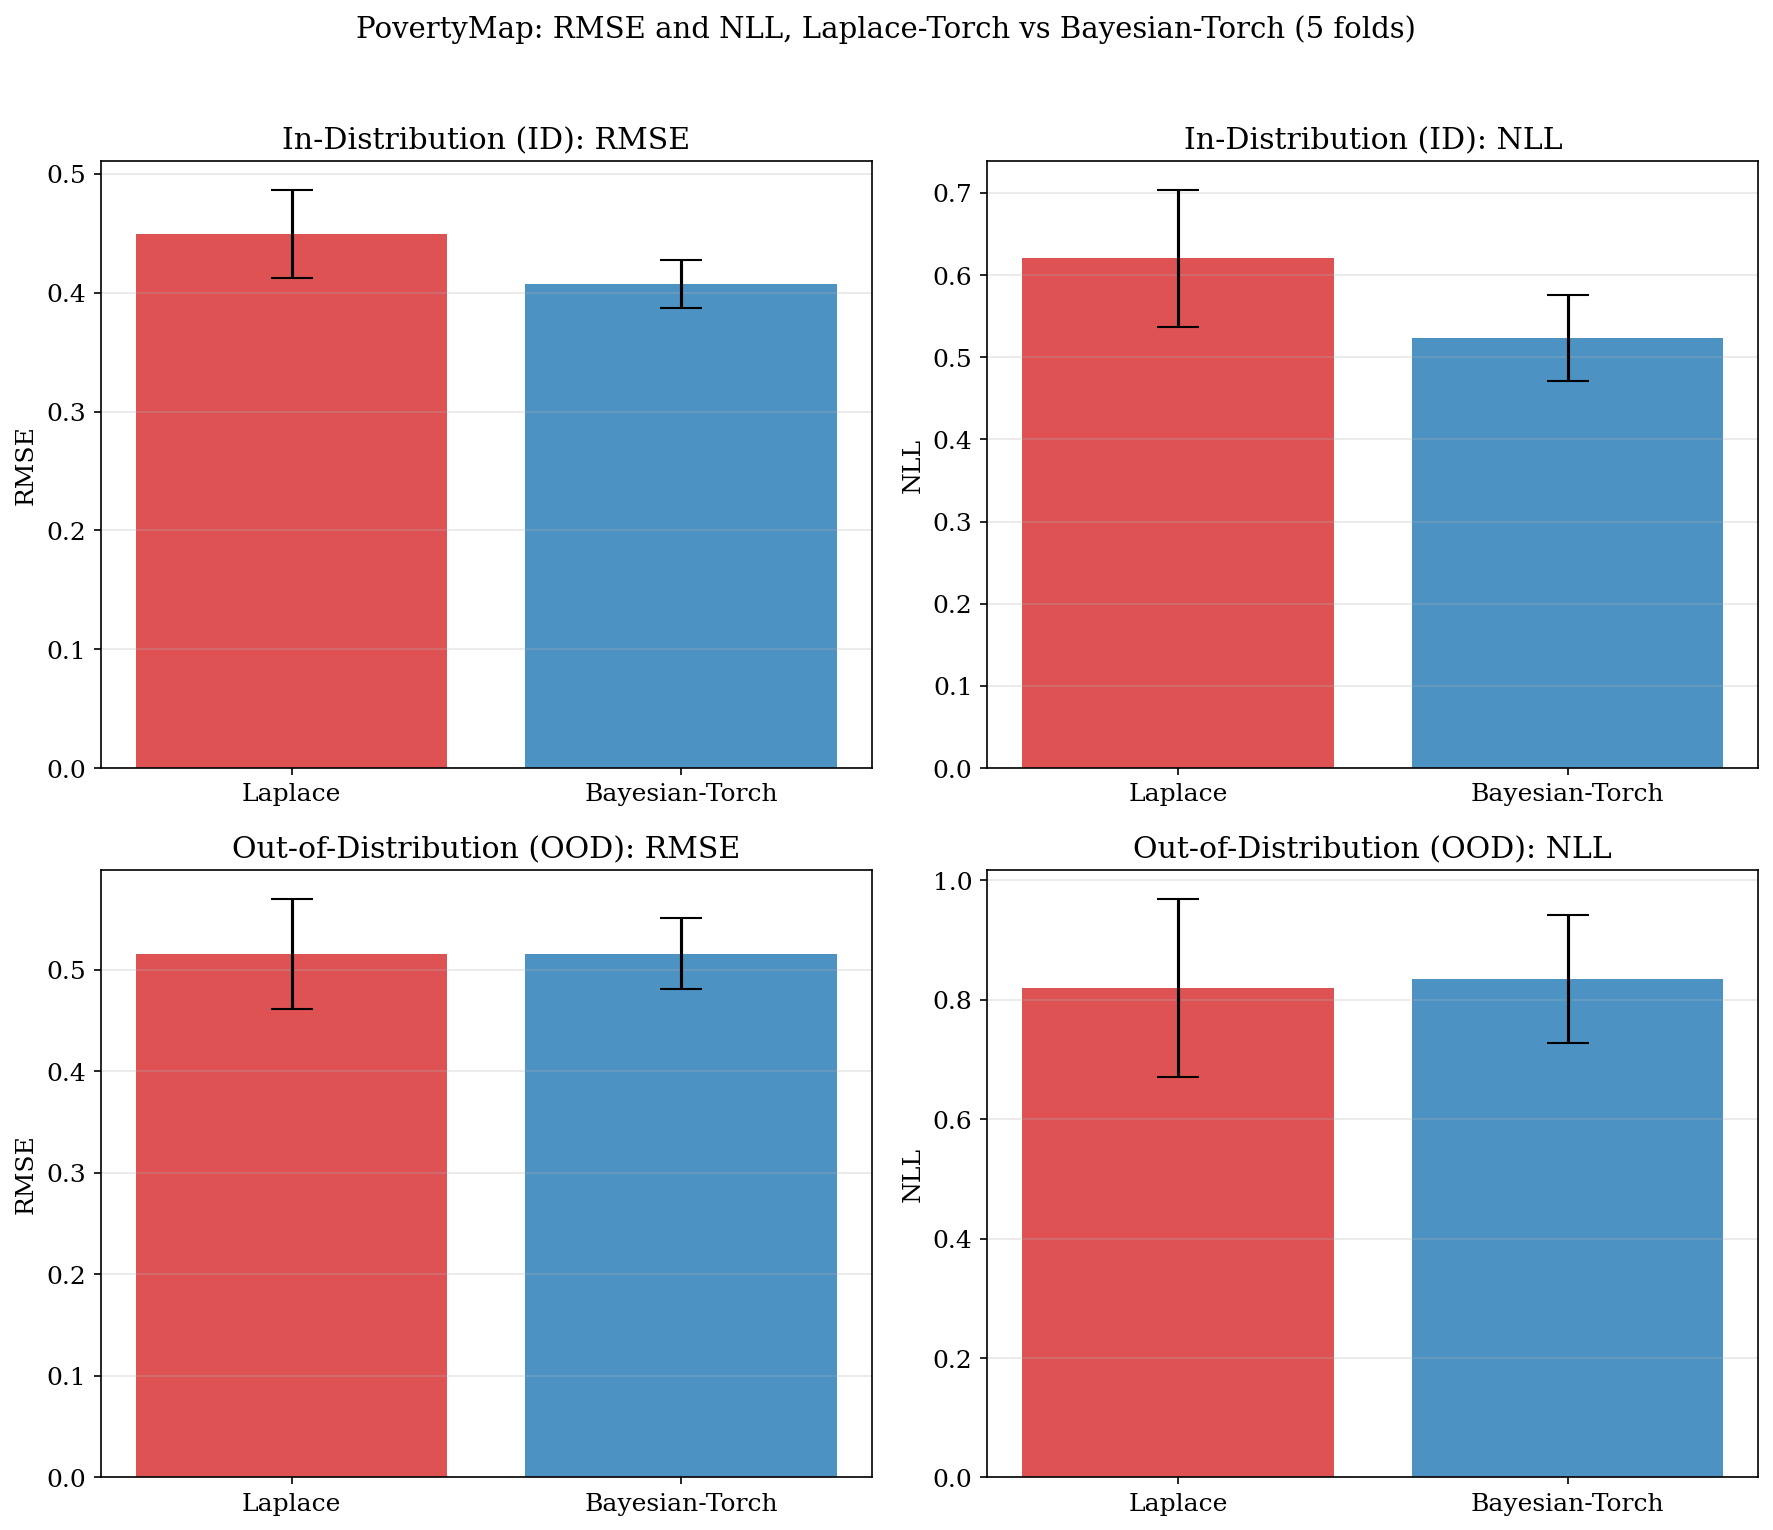
\includegraphics[width=\linewidth]{povertymap_rmse_nll_bar.png}
\caption{PovertyMap RMSE and NLL, ID and OOD, both methods (5 folds).}
\label{fig:pm_rmse_nll_bar}
\end{figure}

% conference papers do not normally have an appendix

\clearpage
% references section
\bibliographystyle{plainnat}
\bibliography{bib.bib}


% that's all folks
\end{document}
